\chapter{Functional Progression Prediction: Results and Discussion}
\label{ch:study1_results}

% ============================================================
\section{Cohort and Target Feasibility}
\label{sec:results_cohort}
% ============================================================

\subsection{Eligibility by Horizon}
\label{subsec:results_eligibility}
Starting from $N\!=\!5{,}436$ subjects with at least one ALSFRS-R record in the PRO-ACT database, the effective cohort size is determined by the availability of follow-up measurements within each target-horizon window (Table~\ref{tab:eligibility}).

For the \textbf{6-month horizon} ($H\!=\!180 \pm 7$\,d), the final dataset contains $N\!=\!1{,}392$ subjects (25.6\% of the initial pool), partitioned into DEV ($n\!=\!1{,}113$, 80\%) and TEST ($n\!=\!279$, 20\%).
For the \textbf{3-month horizon} ($H\!=\!90 \pm 7$\,d), $N\!=\!2{,}407$ subjects (44.3\%) are eligible, split into DEV ($n\!=\!1{,}925$) and TEST ($n\!=\!482$).
A total of 720 subjects are eligible at both horizons.
The substantial attrition from 5{,}436 to 1{,}392 at 6 months reflects two structural properties of the PRO-ACT database:
(i)~many clinical trials had follow-up periods shorter than 180~days, so subjects were never assessed near the 6-month mark;
and (ii)~ALS patients who deteriorated rapidly may have dropped out, been transferred to palliative care, or died before the 180-day window, creating informative censoring that disproportionately removes fast progressors.
Consequently, the 6-month cohort is likely enriched for slower-progressing subjects relative to the full PRO-ACT population, a caveat that should be borne in mind when interpreting the results.
Nevertheless, the 6-month horizon provides greater temporal support for slope estimation (99.8\% based on $\geq 3$ data points, median 7) than the 3-month horizon.

\begin{table}[ht!]
\centering
\caption[Cohort size by prediction horizon]{Cohort size and data partition by prediction horizon.}
\label{tab:eligibility}
\small
\begin{tabular}{lcccc}
\toprule
Horizon & $N$ & \% of PRO-ACT & DEV & TEST \\
\midrule
3 months & 2{,}407 & 44.3\% & 1{,}925 & 482 \\
6 months & 1{,}392 & 25.6\% & 1{,}113 & 279 \\
\bottomrule
\end{tabular}
\end{table}

\subsection{Target Definition and Slope Distribution}
\label{subsec:results_target_summary}
For each subject, functional progression is quantified as the ALSFRS-R slope between baseline and the target horizon, expressed in points per 30~days (see Section~\ref{sec:methods_slope}).
Negative slopes indicate functional decline; the more negative, the faster the deterioration.

The distribution of slopes is left-skewed for both horizons:
\begin{itemize}
  \item \textbf{6-month:} mean $= -0.95 \pm 0.89$\,pts/30d, median $= -0.80$, range $[-5.23,\; +0.85]$.
  \item \textbf{3-month:} mean $= -0.90 \pm 1.16$\,pts/30d, median $= -0.68$, range $[-7.79,\; +2.16]$.
\end{itemize}
The 3-month slopes exhibit higher variance ($\sigma = 1.16$ vs $0.89$), consistent with fewer data points per slope estimate and wider measurement noise over a shorter observation window.
Despite this, 90.5\% of 3-month slopes are based on $\geq 3$ ALSFRS-R measurements (median $n_{\text{points}} = 4$), and 99.8\% of 6-month slopes use $\geq 3$ points (median $n_{\text{points}} = 7$), confirming adequate estimation quality for both horizons.

The binary target (\textit{rapid} vs \textit{slow}) is derived \textbf{fold-wise} during cross-validation by labelling the worst 30\% slopes in the \emph{training} fold as \textit{rapid}.
For the 6-month horizon, the global 30th percentile corresponds to a slope of $-1.25$\,pts/30d; in practice, the fold-wise cutoffs range from $-1.27$ to $-1.19$ (mean $-1.24$), identifying subjects who are declining by more than approximately one ALSFRS-R point per month.

\subsection{Feature Coverage}
\label{subsec:results_coverage}
Feature availability varies substantially across blocks (Table~\ref{tab:feature_coverage}).
The baseline block has effectively complete coverage: ALSFRS-R total and sex are available for 100\% of subjects, while age is present for 87.1\% ($n\!=\!1{,}212$).
The 180 subjects without recorded age correspond to clinical trials in which age was not collected or was anonymised; because this missingness is administrative rather than outcome-dependent, median imputation is applied without risk of introducing prognostic bias.
Vital signs are available for 80.6\% of subjects at a block level ($n\!=\!1{,}122$), with individual features ranging from 44.9\% (height) to 79.2\% (weight).
FVC data are available for 56.3\% (litres) to 54.5\% (percent of normal), motivating the missingness analysis in Section~\ref{sec:results_fvc_missingness}.
At block level, 60.7\% of subjects ($n\!=\!845$) have at least one non-missing FVC feature.
Study arm is recorded for 91.1\% of subjects. The derived riluzole indicator and concomitant-medication count contain no missing values because subjects without a qualifying pre-baseline record are coded as zero.
Labs are moderately available (creatinine: 64.7\%, ALT: 69.0\%).


\begin{table}[ht]
\centering
\caption[Feature coverage, 6-month cohort]{Feature coverage for the 6-month cohort ($N\!=\!1{,}392$). Block-level coverage indicates the fraction of subjects with at least one non-missing feature in the block.}
\label{tab:feature_coverage}
\small
\begin{tabular}{lcc}
\toprule
Feature Block & Features ($n$) & Coverage (\%) \\
\midrule
Baseline (demographics + ALSFRS-R) & 15 & $\sim$100 \\
Vitals & 12 & 80.6 \\
FVC & 3 & 60.7 \\
Treatment & 3 & $\sim$100 \\
Labs & 2 & 64.7--69.0 \\
\midrule
All features & 35 & 100\textsuperscript{$\dagger$} \\
\bottomrule
\multicolumn{3}{l}{\footnotesize $\dagger$After median imputation, all subjects have complete feature vectors.}
\end{tabular}
\end{table}
\break
The heterogeneous coverage across blocks underscores the importance of an imputation strategy that does not introduce outcome-dependent bias, and supports the use of ablation to quantify whether blocks with lower coverage (e.g.\ FVC, Labs) contribute sufficient predictive signal to justify their inclusion.
Note that the dataset contains 39 columns in total, but 4 columns are excluded before modelling: three temporal offsets (\texttt{t0\_delta\_days}, \texttt{vitals\_delta\_days}, \texttt{fvc\_delta\_days}) that encode measurement timing rather than clinical status, and \texttt{ALSFRS\_Responded\_By} which is near-constant ($>$93\% missing).
The remaining 35 features constitute the model input after imputation.


% ============================================================
\section{Data Quality: FVC Missingness Analysis}
\label{sec:results_fvc_missingness}
% ============================================================

FVC in litres is available for 56.3\% of the six-month cohort. Availability shows no clear association with baseline \gls{ALSFRS-R}, age, sex, or the target slope after Bonferroni correction, while the largest observed differences concern study arm ($V=0.357$), \gls{BMI} ($d=0.468$), and medication count ($d=0.332$). This pattern may reflect trial-specific measurement and recording practices, but it does not establish the missing-data mechanism; Appendix~\ref{app:fvc_missingness} reports all eleven comparisons.


% ============================================================
\section{Data Quality: BMI Correction}
\label{sec:results_bmi_fix}
% ============================================================

The plausibility filter described in Section~\ref{sec:methods_bmi_correction} set 132 selected height measurements and 31 weights to missing before \gls{BMI} was recalculated; corrected values in the six-month cohort range from 15.5 to 46.9. The horizon-specific datasets were then regenerated from the cleaned vital-sign features before modelling, with the full audit reported in Appendix~\ref{app:bmi_correction}.


% ============================================================
\section{Exploratory Analysis: Treatment vs Disease Progression}
\label{sec:results_eda_treatment}
% ============================================================

Three treatment-related features are available: clinical trial arm, documented pre-baseline riluzole use, and the number of concomitant medications. Active and Placebo participants have rapid-progression rates of 26.5\% and 31.6\%, respectively, but neither the binary comparison ($\chi^2=3.62$, $p=0.057$) nor the continuous slope comparison ($U=200{,}472$, $p=0.229$) provides evidence of a difference at $\alpha=0.05$. The corresponding rates for participants with and without documented riluzole use are 30.8\% and 28.6\%; again, the binary ($p=0.416$) and continuous ($p=0.534$) comparisons are not statistically significant.

Medication burden and individual drug rates vary across the descriptive groups, but these unadjusted comparisons cannot distinguish pharmacological effects from differences in comorbidity, symptom management, trial procedures, or recording density. The three variables are therefore retained as candidate predictors of patient and trial heterogeneity, with their incremental contribution assessed through feature ablation. Appendix~\ref{app:treatment_eda} reports the complete distributions, subgroup rates, and medication summaries.

% ============================================================
\section{Unified Optuna Hyperparameter Tuning (6-Month Horizon)}
\label{sec:results_optuna_v2}
% ============================================================

Seven model families were tuned with Optuna (60 trials per configuration, \gls{TPE} sampler, seed~42) using subject-wise GroupKFold ($K\!=\!5$), fold-wise binary label definition, and the \gls{DEV} partition only ($n\!=\!1{,}113$).
The seven families---Logistic Regression, Decision Tree, \gls{KNN}, \gls{SVM}, Random Forest, \gls{LGBM}, and \gls{XGB}---were chosen to span linear, distance-based, kernel-based, single-tree, and ensemble paradigms, allowing a systematic comparison across model complexity levels.
Each model was evaluated in both \textbf{unbalanced} and \textbf{balanced} modes---except \gls{KNN}, which lacks native class-weight support, yielding 13 configurations in total.
The objective metric was \gls{PR-AUC} (average precision). After each search, \gls{ROC-AUC} and threshold-dependent metrics ($F_1$, $F_2$ at threshold~0.5) were collected for the selected configuration.
The complete search spaces, trial diagnostics, execution-time summary, and selected parameters are reported in Appendix~\ref{app:tuning}.

Table~\ref{tab:step5v2_tuning} and Figure~\ref{fig:prauc_barchart} summarise the results.

\begin{table}[ht]
\centering
\caption[Optuna-tuned model comparison, 6-month horizon]{Optuna-tuned model comparison (6-month horizon, DEV set, GroupKFold $K\!=\!5$, 60 trials). Models ranked by PR-AUC. Best value per metric in \textbf{bold}.}
\label{tab:step5v2_tuning}
\small
\begin{tabular}{llcccc}
\toprule
Model & Mode & PR-AUC & ROC-AUC & F1\textsubscript{@0.5} & F2\textsubscript{@0.5} \\
\midrule
XGBoost & unbalanced & \textbf{0.434 $\pm$ 0.049} & 0.615 & 0.121 & 0.085 \\
RandomForest & unbalanced & 0.431 $\pm$ 0.042 & 0.610 & 0.023 & 0.015 \\
SVM & balanced & 0.425 $\pm$ 0.049 & \textbf{0.621} & 0.017 & 0.011 \\
RandomForest & balanced & 0.425 $\pm$ 0.046 & 0.615 & 0.442 & 0.480 \\
XGBoost & balanced & 0.424 $\pm$ 0.040 & 0.604 & 0.420 & 0.454 \\
LightGBM & balanced & 0.418 $\pm$ 0.036 & 0.615 & 0.443 & 0.499 \\
LightGBM & unbalanced & 0.415 $\pm$ 0.046 & 0.613 & 0.084 & 0.058 \\
LogisticRegression & balanced & 0.407 $\pm$ 0.051 & 0.611 & \textbf{0.462} & \textbf{0.527} \\
DecisionTree & balanced & 0.404 $\pm$ 0.054 & 0.606 & 0.434 & 0.514 \\
LogisticRegression & unbalanced & 0.401 $\pm$ 0.054 & 0.607 & 0.041 & 0.028 \\
SVM & unbalanced & 0.389 $\pm$ 0.057 & 0.594 & 0.032 & 0.021 \\
DecisionTree & unbalanced & 0.388 $\pm$ 0.046 & 0.605 & 0.329 & 0.293 \\
KNeighbors & unbalanced & 0.387 $\pm$ 0.055 & 0.587 & 0.035 & 0.022 \\
\bottomrule
\end{tabular}
\end{table}


\begin{figure}[ht!]
  \centering
  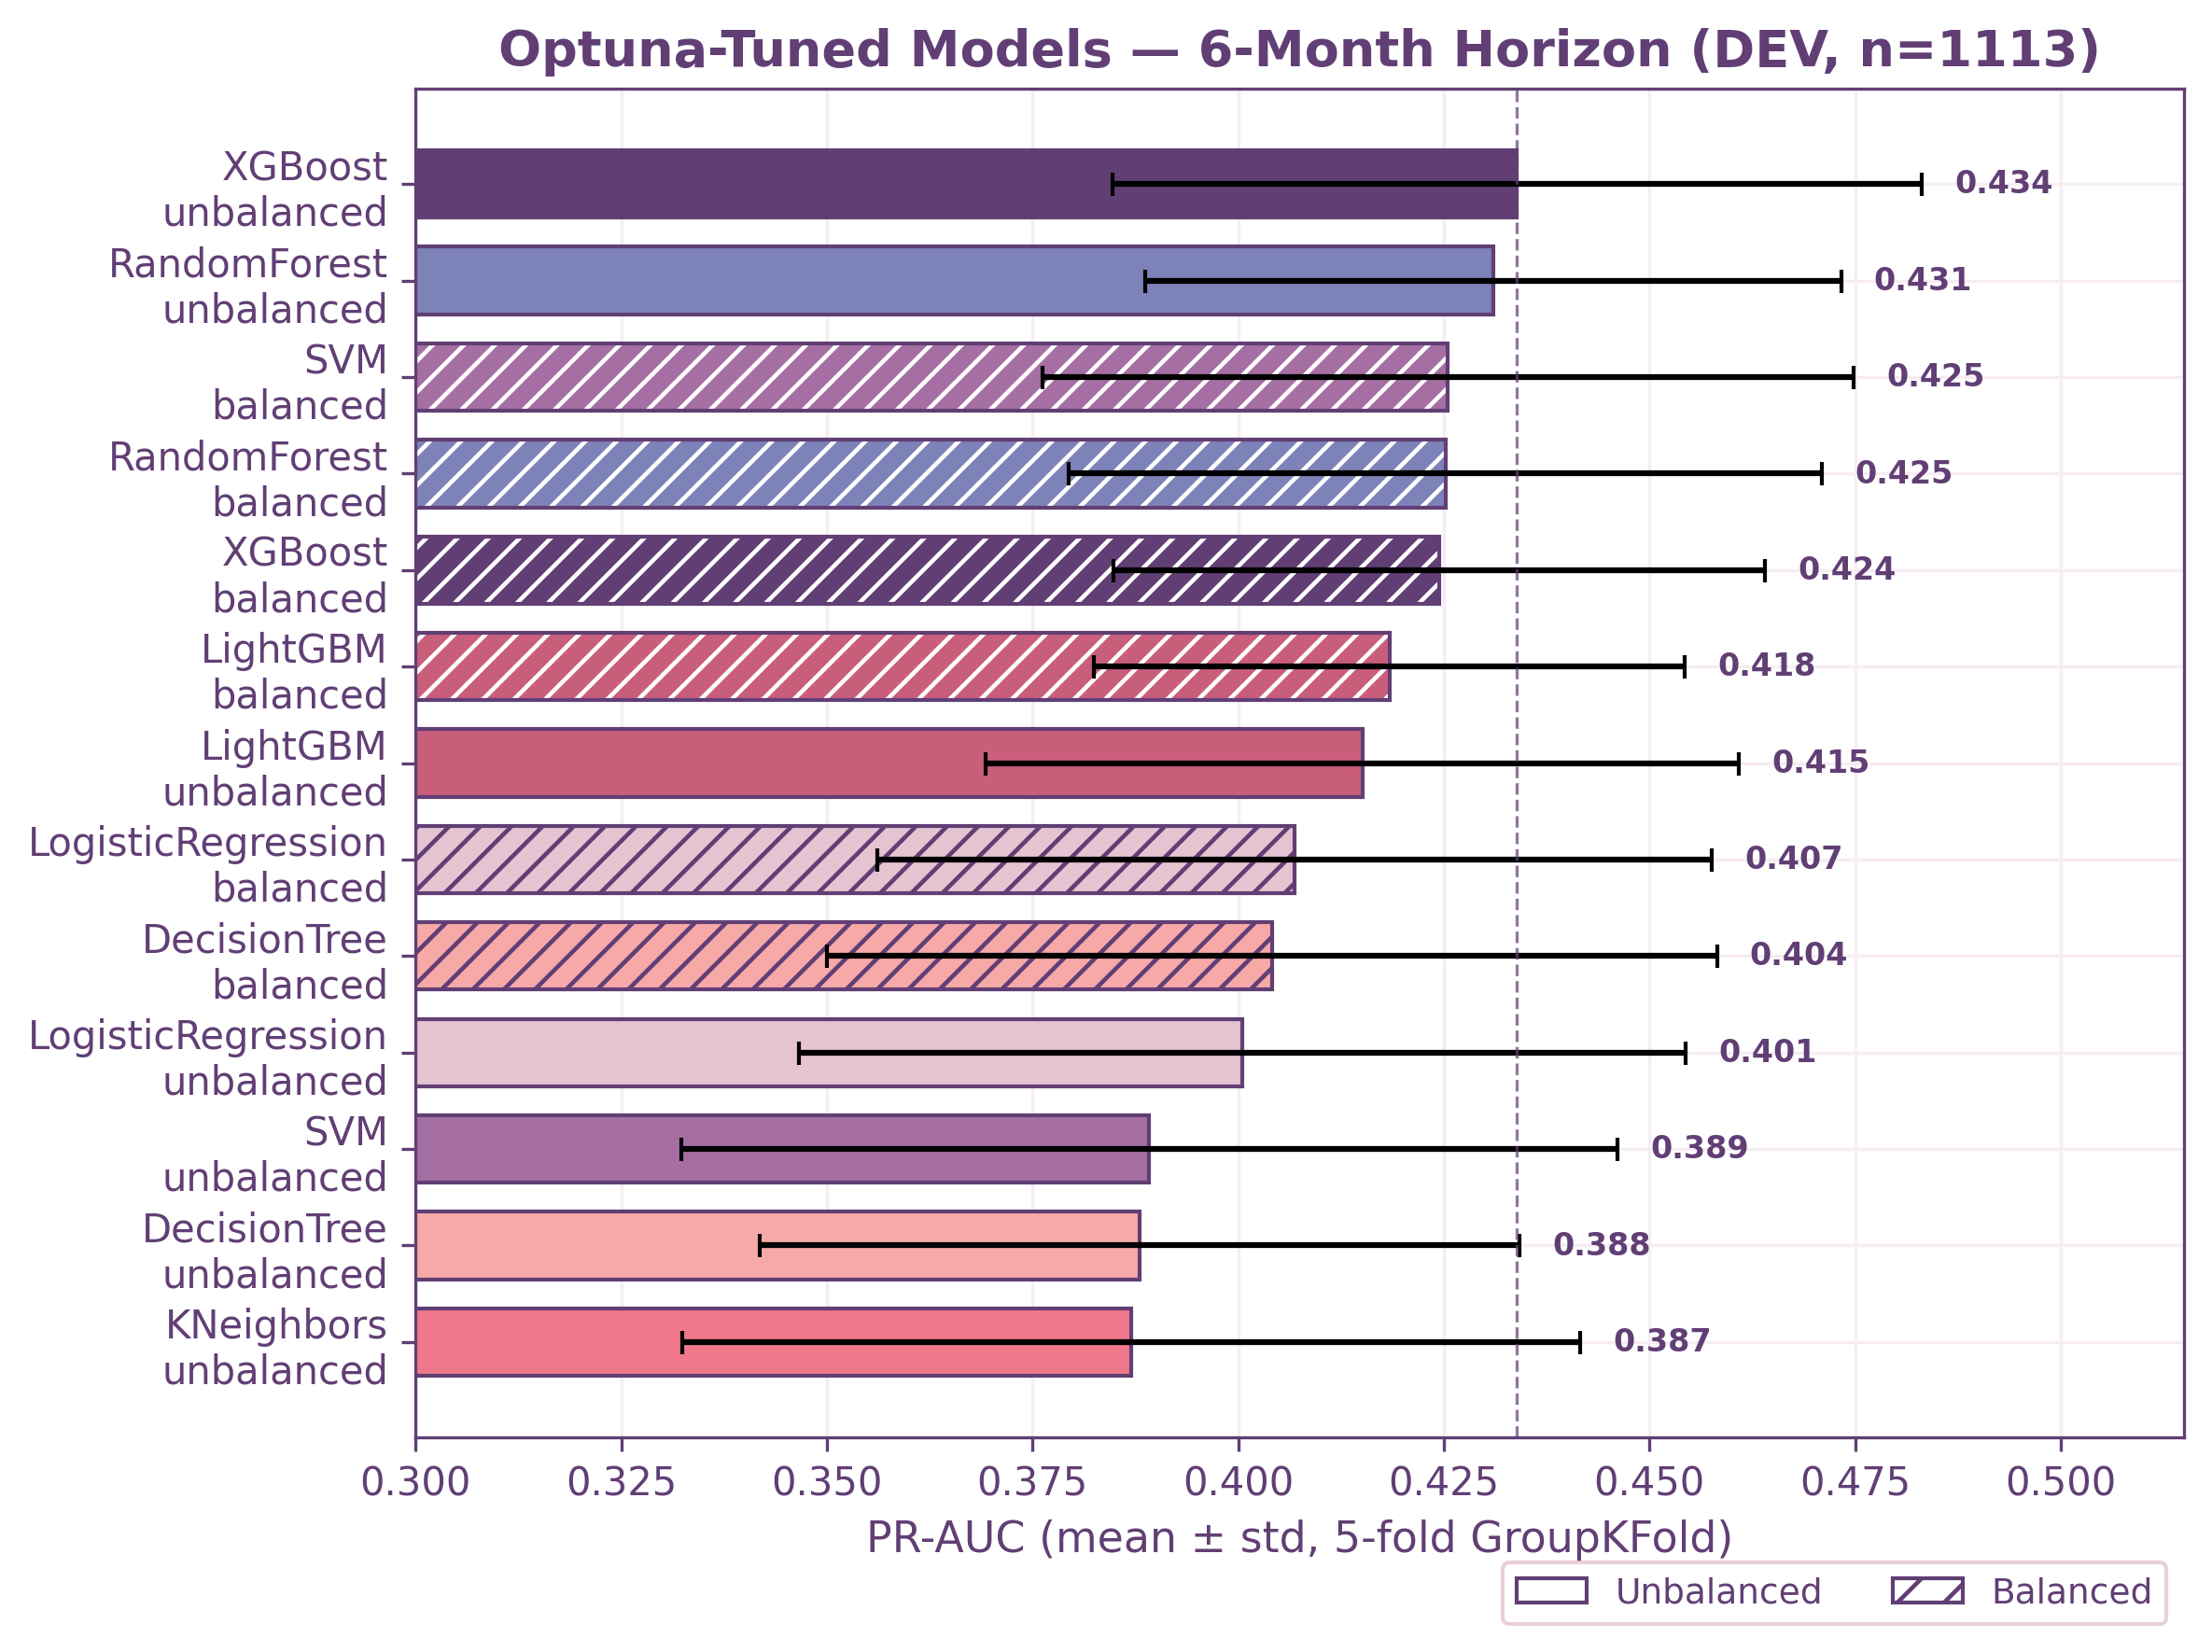
\includegraphics[width=0.95\linewidth]{images/figures/step5v2_prauc_barchart.png}
  \caption[Cross-validation PR-AUC by model, 6-month]{PR-AUC comparison of Optuna-tuned models (6-month, DEV). Blue bars: unbalanced mode; orange bars: balanced mode. Error bars show $\pm 1$ standard deviation across 5 folds.}
  \label{fig:prauc_barchart}
\end{figure}

\clearpage
\noindent\textbf{Key observations.}
\begin{enumerate}
  \item \textbf{Top-ranked model.} XGBoost (unbalanced) achieves the highest PR-AUC ($0.434 \pm 0.049$), closely followed by Random Forest (unbalanced, $0.431 \pm 0.042$) and SVM (balanced, $0.425 \pm 0.049$).
    The small differences among the leading configurations show that several model families achieve similar internal validation performance; they do not, by themselves, establish a performance ceiling.
  \item \textbf{Effect of class balancing on PR-AUC.} Weighting produces small changes for Random Forest ($0.431 \to 0.425$), LightGBM ($0.415 \to 0.418$), and XGBoost ($0.434 \to 0.424$). The largest change occurs for SVM, whose PR-AUC increases from $0.389$ to $0.425$. The effect is therefore model-dependent rather than uniformly beneficial or detrimental.
  \item \textbf{Threshold-dependent metrics.} At the default threshold of 0.5, $F_1$ and $F_2$ are low for most unbalanced models, although Decision Tree is a clear exception. Weighting substantially increases these scores for Decision Tree, Random Forest, Logistic Regression, LightGBM, and XGBoost; for example, Logistic Regression $F_2$ increases from $0.028$ to $0.527$. Balanced SVM remains near zero at this cutoff despite its improved PR-AUC.
  \item \textbf{Interpretable baselines.} Logistic Regression balanced ($\text{PR-AUC} = 0.407$) performs only $0.027$ below XGBoost unbalanced, making it a competitive interpretable alternative.
    Its coefficients can be directly analysed to understand feature directionality.
\end{enumerate}


% ────────────────────────────────────────────────────────────
\subsection{Balanced vs Unbalanced: Paired Comparison}
\label{subsec:results_bal_vs_unbal}
% ────────────────────────────────────────────────────────────

Figure~\ref{fig:bal_vs_unbal} presents a paired (dumbbell) comparison of PR-AUC and ROC-AUC for each model family across the two class-weighting modes.
The differences between modes are approximately 0.01 or less for Random Forest, LightGBM, and XGBoost. Decision Tree improves by 0.016 with weighting, while Logistic Regression changes by 0.006. SVM shows the largest difference, increasing by 0.036 in balanced mode. Thus, class weighting has little effect on ranking performance for most model families in this experiment, but the SVM result shows that this cannot be assumed for every classifier.

The larger differences in $F_1$ and $F_2$ describe how class weighting changes predictions at the common threshold of 0.5; Section~\ref{sec:results_threshold_xgb} evaluates the operating threshold selected for XGBoost.

\begin{figure}[ht!]
  \centering
  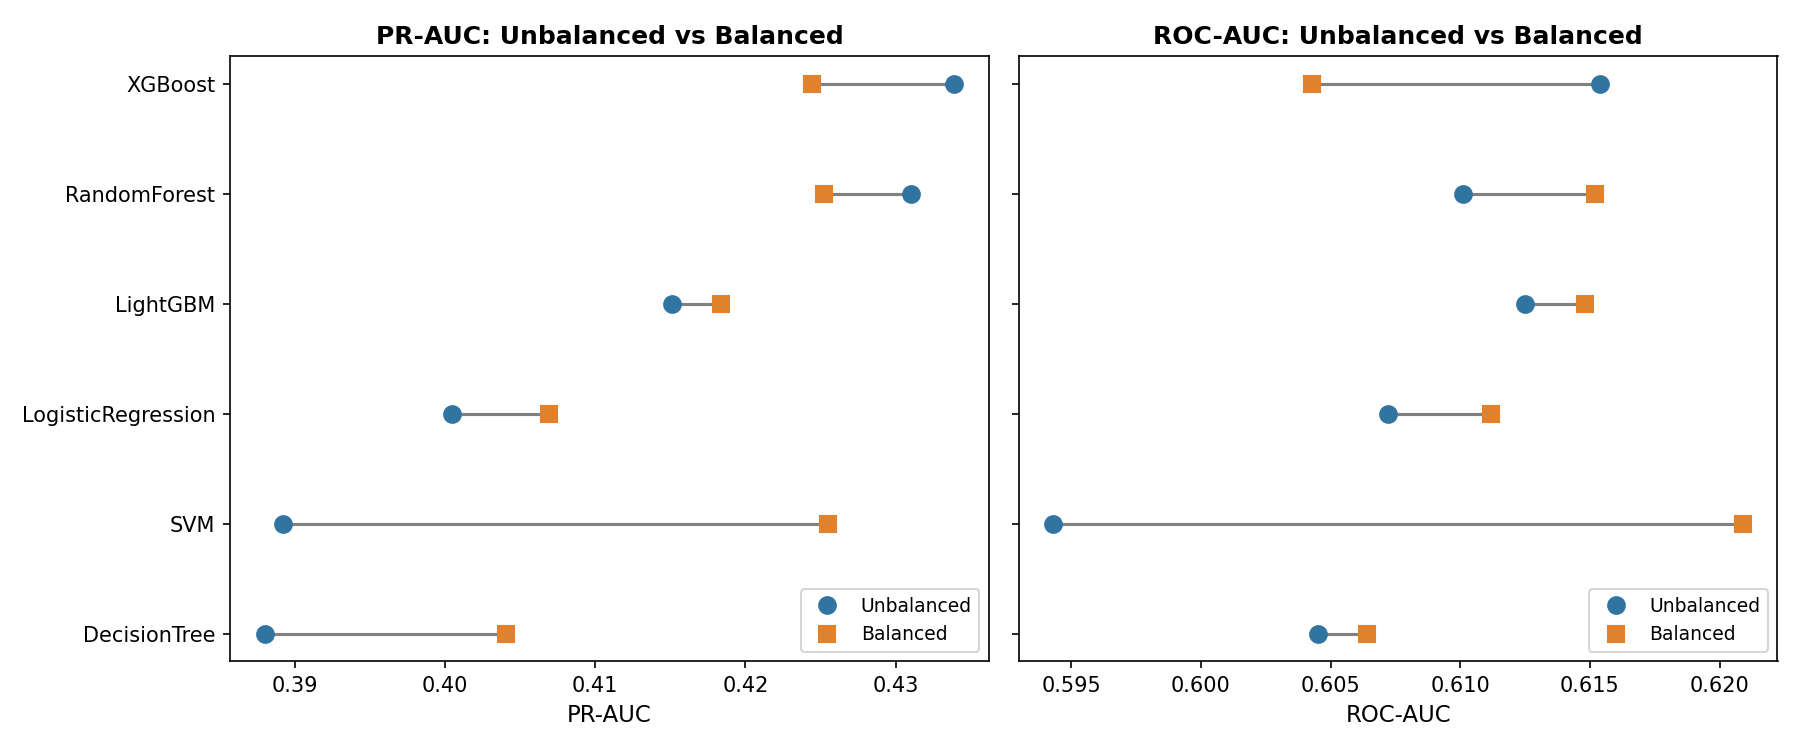
\includegraphics[width=0.95\linewidth]{images/figures/step5v2_balanced_vs_unbalanced.png}
  \caption[Balanced vs.\ unbalanced mode comparison]{Paired comparison of unbalanced ($\circ$) vs balanced ($\square$) modes for each model. Left panel: PR-AUC; right panel: ROC-AUC. Lines connect the same model across both modes.}
  \label{fig:bal_vs_unbal}
\end{figure}


% ────────────────────────────────────────────────────────────
\subsection{Metric Rank Correlation}
\label{subsec:results_metric_correlation}
% ────────────────────────────────────────────────────────────

We computed Spearman rank correlations between all pairs of cross-validated evaluation metrics across the 13 model $\times$ mode configurations to compare the resulting model rankings.
If two metrics produce highly correlated model rankings, they provide redundant information; if uncorrelated, they capture different aspects of model behaviour.

The correlations quantify agreement between rankings but do not make the metrics interchangeable, since each captures a different aspect of performance. Two patterns are visible:
\begin{itemize}
  \item \textbf{Threshold-free metrics:} PR-AUC and ROC-AUC are strongly correlated ($\rho\!=\!0.758$, $p\!=\!0.003$), indicating that models which rank probability predictions well under one curve generally rank well under the other.
    The two measures therefore produce broadly similar, although not identical, model rankings.
  \item \textbf{Threshold-dependent metrics at fixed cutoff:} $F_1$ and $F_2$ at threshold~0.5 are almost perfectly correlated with each other ($\rho\!=\!0.984$, $p < 0.001$), while neither shows evidence of a monotonic association with PR-AUC ($|\rho| < 0.08$, $p > 0.8$).
    In these configurations, the fixed-threshold metrics are strongly influenced by whether predicted probabilities cross 0.5 and do not reproduce the ranking obtained from the full probability curves.
\end{itemize}

These findings support the use of PR-AUC as the primary model-selection metric in this imbalanced classification setting. $F_1$ and $F_2$ become informative for the intended operating point only after the threshold has been selected on development data (Section~\ref{sec:results_threshold_xgb}). The complete metric heatmap is provided in Appendix~\ref{app:tuning_diagnostics}.


\clearpage 
% ============================================================
\section{Feature Block Ablation}
\label{sec:results_ablation_v2}
% ============================================================

The feature-block analysis applies the hyperparameters tuned on the full feature set to each reduced configuration. It therefore describes the sensitivity of each fitted model family to the available feature blocks without re-optimising the model for every subset.

Four selected model configurations were evaluated across six feature configurations:
\textbf{A}~(core baseline variables, $n\!=\!15$),
\textbf{B}~(A + vitals, $n\!=\!27$),
\textbf{C}~(A + FVC, $n\!=\!18$),
\textbf{D}~(A + vitals + FVC, $n\!=\!30$),
\textbf{E}~(D + treatment, $n\!=\!33$),
\textbf{F}~(full set with labs, $n\!=\!35$).
Blocks B and C are parallel extensions of A rather than consecutive steps. D combines both blocks, while E and F then add treatment and laboratory variables sequentially.

Figure~\ref{fig:ablation_v2} compares the PR-AUC profile across feature configurations for each model.

\begin{figure}[ht!]
  \centering
  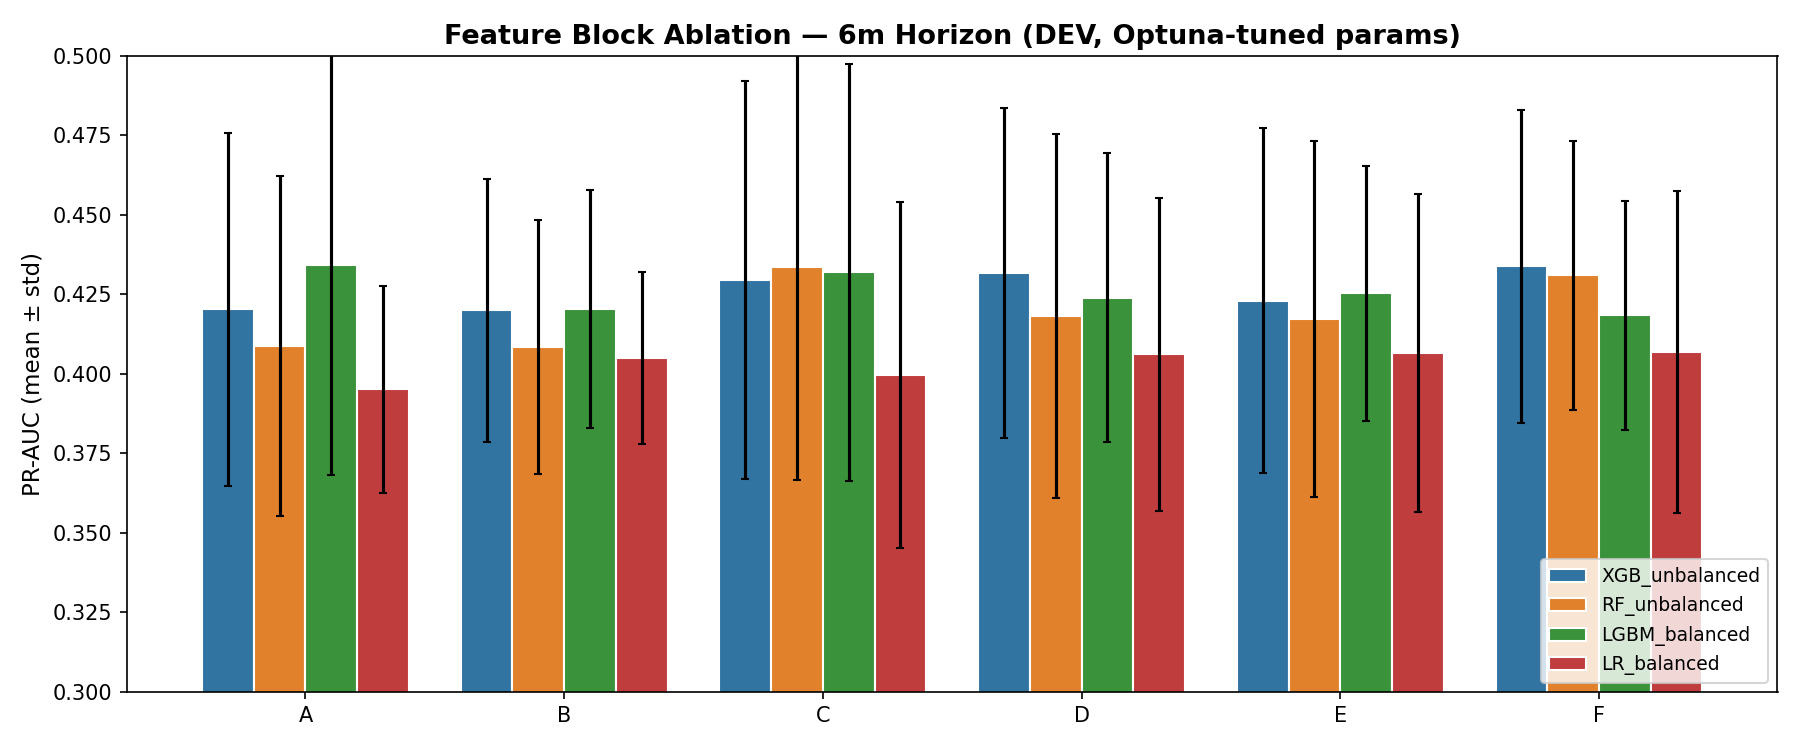
\includegraphics[width=0.85\linewidth]{images/figures/step5v2_ablation_prauc.png}
  \caption[Feature block ablation PR-AUC curves]{Feature-block analysis on the six-month DEV set using hyperparameters tuned on the full feature configuration. Points show mean PR-AUC and error bars show the standard deviation across five folds. B and C are alternative extensions of A; D combines both before treatment and laboratory variables are added in E and F.}
  \label{fig:ablation_v2}
\end{figure}

The core baseline variables retain most of the observed discrimination. Their PR-AUC ranges from 0.395 for Logistic Regression to 0.434 for LightGBM, and the best configuration within each model improves on this block by no more than 0.025. FVC produces the clearest additional signal for the unbalanced tree ensembles: adding it to baseline raises Random Forest from 0.409 to 0.434 and XGBoost from 0.420 to 0.430. The corresponding change is smaller for Logistic Regression and slightly negative for LightGBM, so the effect is not shared uniformly across model families.

Vital signs, treatment variables, and laboratory measurements produce smaller and less consistent changes. The full feature set is best for XGBoost (0.434) and Logistic Regression (0.407), while Random Forest peaks with baseline plus FVC (0.434) and LightGBM with baseline alone (0.434). These differences are small relative to the fold standard deviations and were not tested separately. The analysis therefore supports the prognostic relevance of FVC~\cite{Papaiz2022}, but does not show that adding every available block improves the classifier. Appendix~\ref{app:ablation} reports the complete numerical results.


% ============================================================
\section{Cross-Horizon Comparison: 3 vs 6 Months}
\label{sec:results_3m}
% ============================================================

The four highest-ranked six-month model families were tuned independently on the three-month DEV set ($n\!=\!1{,}925$), in balanced and unbalanced modes. Balanced XGBoost achieved the highest three-month PR-AUC ($0.426 \pm 0.036$), followed by unbalanced XGBoost and unbalanced LightGBM (both 0.423). The leading four configurations differed by less than 0.004, well within their fold-to-fold variation. Complete three-month results are reported in Appendix~\ref{app:three_month}.

Figure~\ref{fig:3m_vs_6m_grouped} compares the eight matched model configurations across horizons.

\begin{figure}[H]
  \centering
  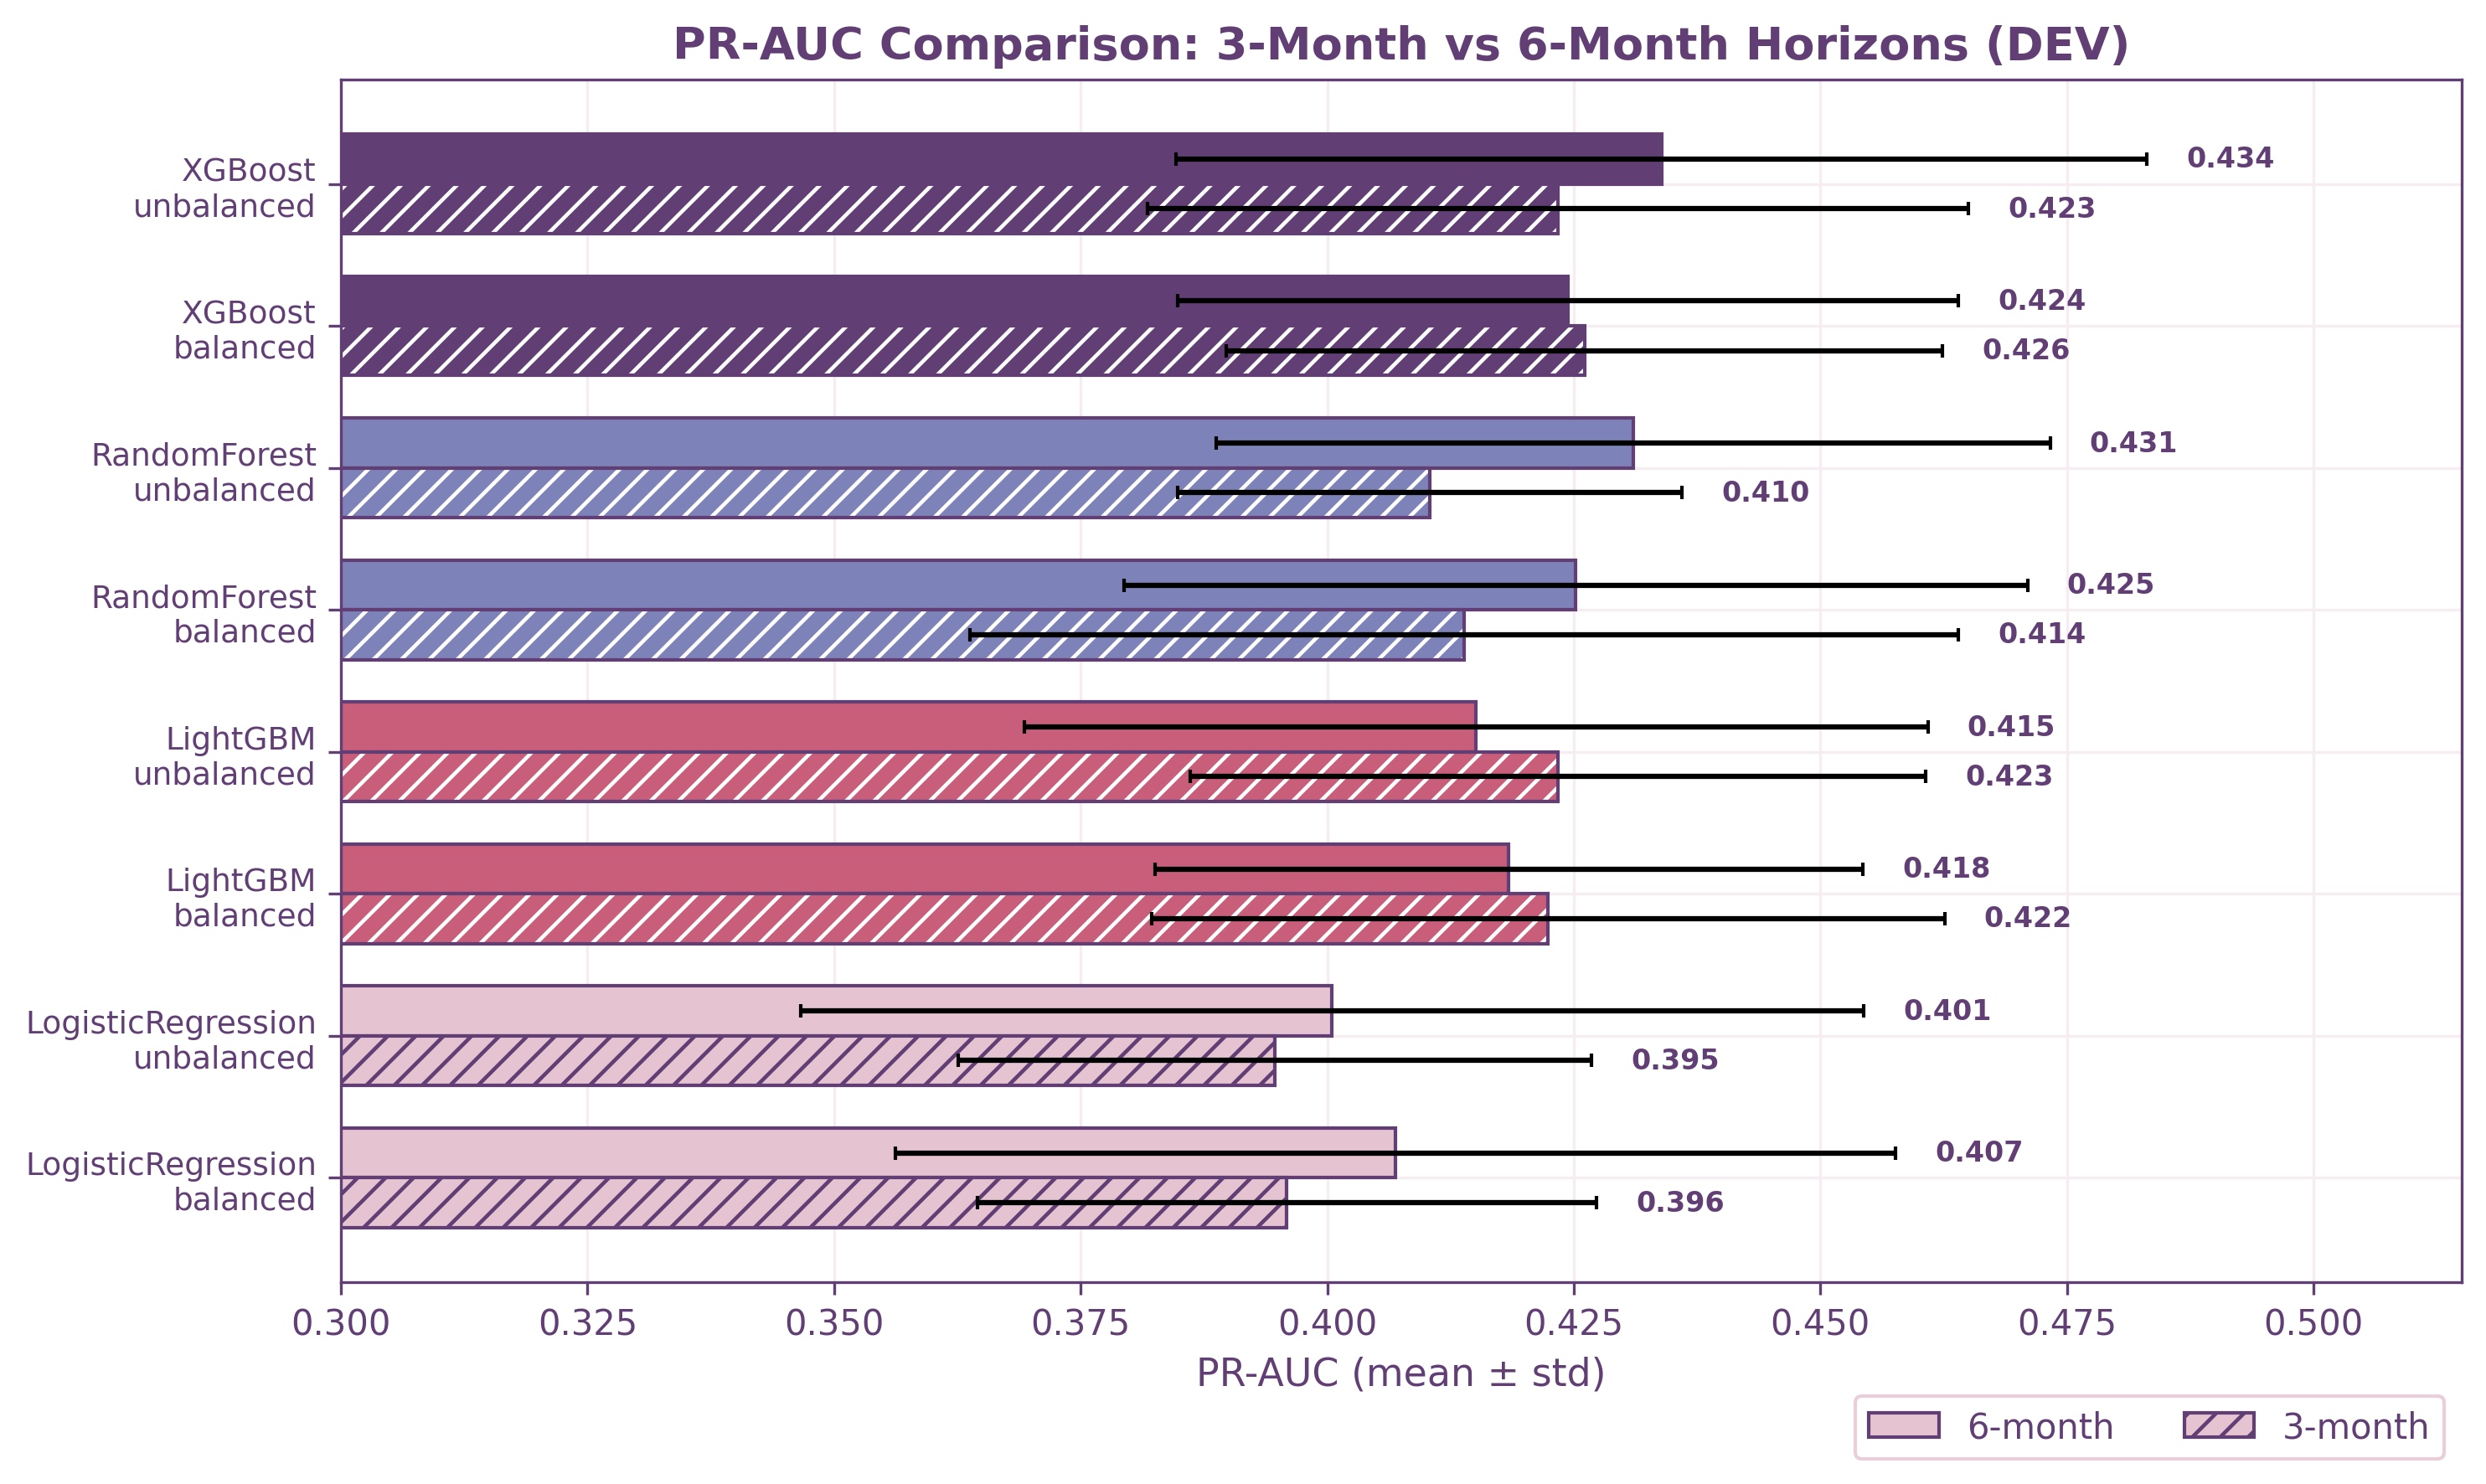
\includegraphics[width=0.95\linewidth]{images/figures/step5v2_3m_vs_6m_prauc.png}
  \caption[PR-AUC comparison: 3-month vs.\ 6-month]{Descriptive PR-AUC comparison between 3-month and 6-month horizons for matched model $\times$ mode configurations tuned independently on their respective DEV sets. Annotations show mean PR-AUC values.}
  \label{fig:3m_vs_6m_grouped}
\end{figure}

%\break

Across the eight pairs, absolute PR-AUC differences range from 0.002 to 0.021. Five configurations favour six months and three favour three months; their mean PR-AUC is 0.419 and 0.414, respectively. The largest decrease at three months occurs for unbalanced Random Forest ($\Delta=-0.021$), whereas unbalanced LightGBM has the largest increase ($\Delta=+0.008$). Every difference is smaller than the cross-validation standard deviation of the corresponding configurations. Although all eight models have higher ROC-AUC at three months, PR-AUC changes in both directions, illustrating that conclusions also depend on the selected metric.

XGBoost leads at both horizons, in unbalanced mode at six months and balanced mode at three months. The six-month horizon remains the basis for the subsequent analyses because its slopes use a longer follow-up period and more observations per participant, without a lower overall PR-AUC in the matched comparison. The shorter-horizon results support the pipeline's sensitivity analysis, but the cohorts, folds, and slope estimates differ; they are neither an external validation nor evidence that horizon alone caused the observed changes. Appendix~\ref{app:three_month} provides the full comparison table and scatter plot.


% ============================================================
\section{Statistical Comparison of Models}
\label{sec:results_statistical_comparison}
% ============================================================

The best configuration from each model family was re-evaluated on the same five GroupKFold splits. This produced paired fold-level PR-AUC scores for an exploratory comparison of the seven selected configurations.

\subsection{Per-Fold Performance}

Figure~\ref{fig:step7_fold_boxplot} shows the per-fold PR-AUC distribution for each model.
Mean PR-AUC ranges from 0.434 for unbalanced XGBoost to 0.387 for unbalanced KNN. The fold-level standard deviations range from 0.036 to 0.055, and the distributions overlap across all seven configurations.

\begin{figure}[ht!]
  \centering
  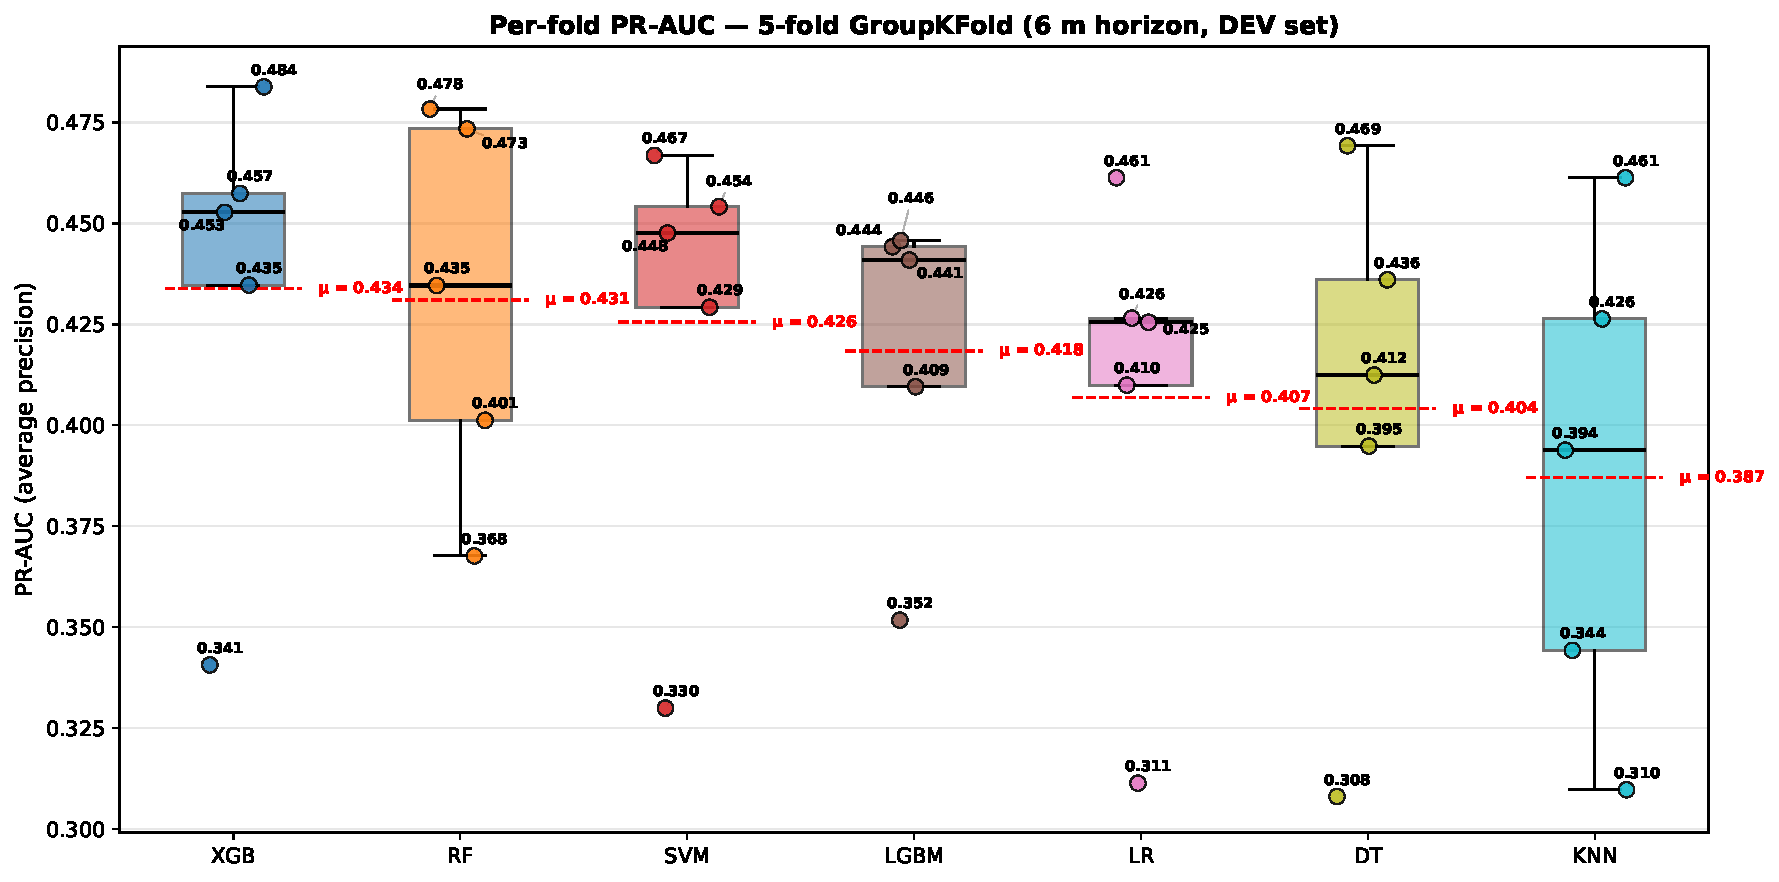
\includegraphics[width=0.88\linewidth]{images/figures/step7_fold_prauc_boxplot.pdf}
  \caption[Per-fold PR-AUC distribution, 5-fold CV]{Per-fold PR-AUC for the seven best-per-family models across 5-fold GroupKFold on the DEV set (6-month horizon).
  Points show individual folds and diamonds mark the mean.
  XGBoost (unbalanced) has the highest mean PR-AUC (0.434), and the distributions overlap across models.}
  \label{fig:step7_fold_boxplot}
\end{figure}

\subsection{Friedman and Pairwise Comparisons}

The Friedman test gives $\chi^2_F(6)=12.43$ and $p=0.053$. The null hypothesis of equal rank distributions is therefore not rejected at $\alpha=0.05$. Kendall's coefficient is $W=0.414$, indicating some agreement among folds in their model rankings, but the five-fold design provides limited power and the asymptotic $p$-value lies close to the chosen threshold.

The exploratory Wilcoxon comparisons are reported in Appendix~\ref{app:stats}. The smallest raw two-sided $p$-value is 0.0625, observed for XGBoost versus Logistic Regression, XGBoost versus Decision Tree, and Random Forest versus KNN. All 21 Bonferroni-adjusted values are 1.0. This result is largely determined by the discrete resolution of a signed-rank test with five pairs and the number of simultaneous comparisons; it should not be interpreted as demonstrating equivalence among the models.

Unbalanced XGBoost remains the selected configuration because it has the highest mean cross-validated PR-AUC under the prespecified selection criterion. Its advantage over unbalanced Random Forest is only 0.003, and the statistical analysis does not establish that this difference is systematic. The selection should therefore be understood as a reproducible ranking decision within this development dataset, rather than evidence that XGBoost is intrinsically superior to the other leading models.


% ============================================================
\section{Threshold Optimisation}
\label{sec:results_threshold_xgb}
% ============================================================

The default threshold of $t\!=\!0.50$ produces very few positive predictions for the selected unbalanced XGBoost model. Alternative thresholds are therefore compared using out-of-fold (\gls{OOF}) predictions from five-fold GroupKFold on the DEV set. Labels for this analysis use the fixed DEV 30th-percentile slope cutoff ($-1.243$ points per 30 days).

Three optimality criteria are evaluated:
\begin{enumerate}
  \item \textbf{$F_2$-optimal} ($t\!=\!0.05$): $F_2=0.682$. At the lower boundary of the threshold grid, all 1,113 DEV participants are classified as rapid, giving recall 1.00 and precision 0.300. This solution provides no separation into predicted classes.
  \item \textbf{$F_1$-optimal} ($t\!=\!0.21$): $F_1=0.479$, with recall 0.874 and precision 0.330. This threshold classifies 79.6\% of DEV as rapid.
  \item \textbf{Youden's~$J$} ($t\!=\!0.35$): $J=0.171$, with recall 0.410 and precision 0.424. This criterion gives equal importance to sensitivity and specificity.
\end{enumerate}

$t=0.21$ is retained as the primary operating point because it maximises $F_1$ within the evaluated grid without collapsing to an all-positive classification. It nevertheless represents an aggressive rule: almost four in five development participants are flagged, and precision is only three percentage points above the rapid-progression prevalence. The threshold is therefore used to evaluate a sensitivity-oriented prototype and is not presented as a clinically established cutoff.
Figure~\ref{fig:step6_threshold_sweep} illustrates the multi-metric threshold sweep.

\begin{figure}[H]
  \centering
  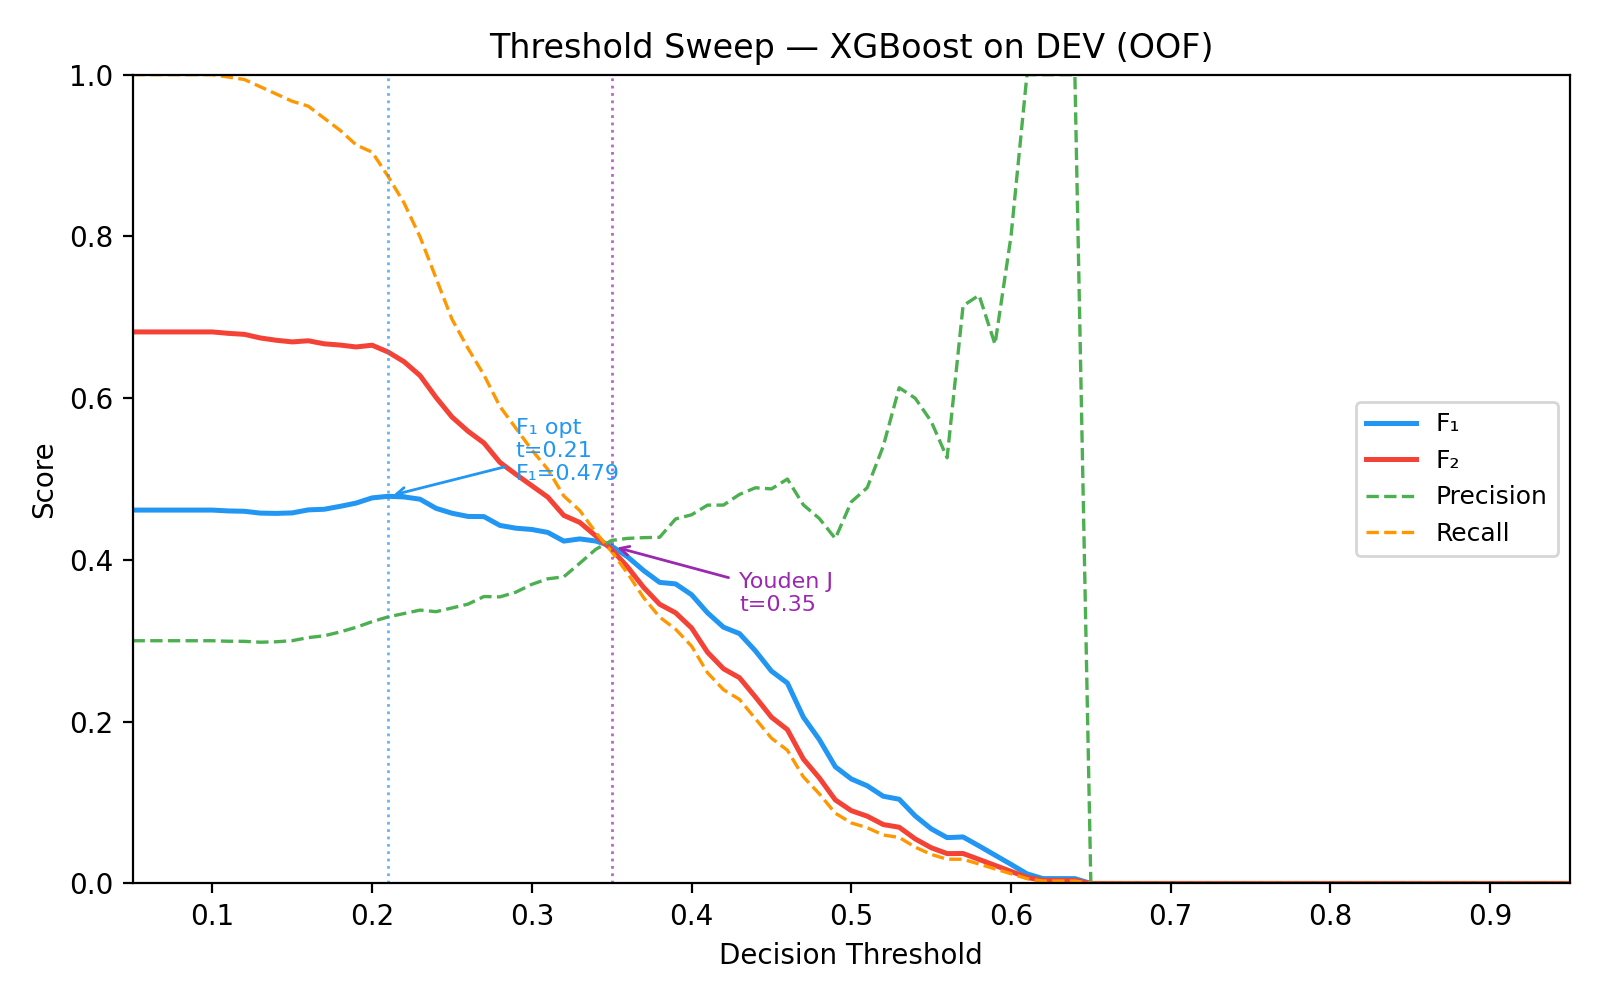
\includegraphics[width=0.70\linewidth]{images/figures/step6_threshold_sweep.png}
  \caption[Threshold sweep on DEV out-of-fold predictions]{Threshold sweep on DEV out-of-fold predictions for XGBoost (unbalanced, 6\,m).
  The $F_1$-optimal threshold ($t\!=\!0.21$, blue dotted) and Youden's~$J$ operating point ($t\!=\!0.35$, purple dotted) are annotated.}
  \label{fig:step6_threshold_sweep}
\end{figure}


% ============================================================
\section{Held-Out Test Set Evaluation}
\label{sec:results_test_eval}
% ============================================================

The seven configurations selected within each model family are fitted on the full DEV partition and evaluated once on the held-out TEST partition ($n\!=\!279$, rapid prevalence $30.1$\%).
Labels are defined using the 30th-percentile slope cutoff computed on the DEV set ($-1.243$~points per 30 days), ensuring no information leaks from the test set into the labelling process.

\clearpage
\subsection{Discrimination Metrics}

Table~\ref{tab:step6_test_metrics} reports threshold-free metrics (PR-AUC, ROC-AUC) and threshold-dependent metrics at the default $t\!=\!0.50$.

\begin{table}[ht!]
\centering
\caption[Held-out TEST set metrics, 6-month]{Held-out TEST set metrics (6-month horizon, $n\!=\!279$) from models fitted on DEV only. PR-AUC and ROC-AUC are threshold-free; $F_1$ and $F_2$ are evaluated at the default $t\!=\!0.50$; the Brier score measures probabilistic error (lower is better).}
\label{tab:step6_test_metrics}
\small
\begin{tabular}{l c c c c c c}
\toprule
Model & Mode & PR-AUC & ROC-AUC & $F_1$ & $F_2$ & Brier \\
\midrule
  RandomForest  & unbal. & \textbf{0.459} & 0.664 & 0.000 & 0.000 & 0.199 \\
  XGBoost       & unbal. & 0.456 & 0.660 & 0.085 & 0.058 & \textbf{0.197} \\
  SVM           & bal.   & 0.447 & \textbf{0.675} & 0.000 & 0.000 & 0.198 \\
  LightGBM      & bal.   & 0.429 & 0.637 & 0.422 & 0.440 & 0.224 \\
  LogisticReg.  & bal.   & 0.421 & 0.671 & \textbf{0.484} & \textbf{0.520} & 0.231 \\
  KNeighbors    & unbal. & 0.393 & 0.583 & 0.046 & 0.029 & 0.206 \\
  DecisionTree  & bal.   & 0.373 & 0.569 & 0.417 & 0.417 & 0.270 \\
\bottomrule
\end{tabular}
\end{table}\hfill

\noindent\textbf{Key observations:}
\begin{enumerate}
  \item \textbf{PR-AUC on held-out data.}
    Random Forest (PR-AUC\,$=\!0.459$) and XGBoost ($0.456$) both score slightly above their cross-validated development means ($0.431$ and $0.434$, respectively). This provides no evidence of a marked performance drop on the TEST partition, although a single held-out estimate cannot establish the absence of overfitting.
  \item \textbf{SVM has the highest ROC-AUC point estimate} ($0.675$), followed closely by Logistic Regression ($0.671$), Random Forest ($0.664$), and XGBoost ($0.660$).
    Its PR-AUC is lower than that of Random Forest and XGBoost, and it produces no positive predictions at $t\!=\!0.50$. The latter reflects an unsuitable default operating threshold rather than an absence of ranking ability.
  \item \textbf{Default threshold is unsuitable for unbalanced models.}
    XGBoost, RF, and KNN (all trained without class weighting) produce near-zero $F_1$ and $F_2$ at $t\!=\!0.50$, because their predicted probabilities concentrate below $0.50$ for the minority class.
    This reinforces the need for threshold optimisation (Section~\ref{sec:results_threshold_xgb}).
  \item \textbf{Class weighting changes default-threshold behaviour.}
    Balanced Logistic Regression achieves the highest $F_1$ ($0.484$) and $F_2$ ($0.520$) at $t\!=\!0.50$. These values describe performance at a common cutoff and do not replace the threshold-free criteria used for model selection.
\end{enumerate}

\noindent\textbf{Relation to model selection.}
XGBoost (unbalanced) had already been selected from the \gls{DEV} results, where it achieved the highest cross-validated PR-AUC. Random Forest obtains the highest TEST PR-AUC by approximately 0.002 using the unrounded estimates (0.459 versus 0.456 as displayed), but the held-out results are not used to repeat model selection. XGBoost therefore remains the prespecified model for the subsequent analyses. Its Brier score ($0.197$) is also the lowest point estimate among the seven TEST evaluations, although it is nearly identical to SVM ($0.198$) and Random Forest ($0.199$).
Figure~\ref{fig:step6_test_prauc_bar} presents a visual comparison of PR-AUC across all models.

\begin{figure}[H]
  \centering
  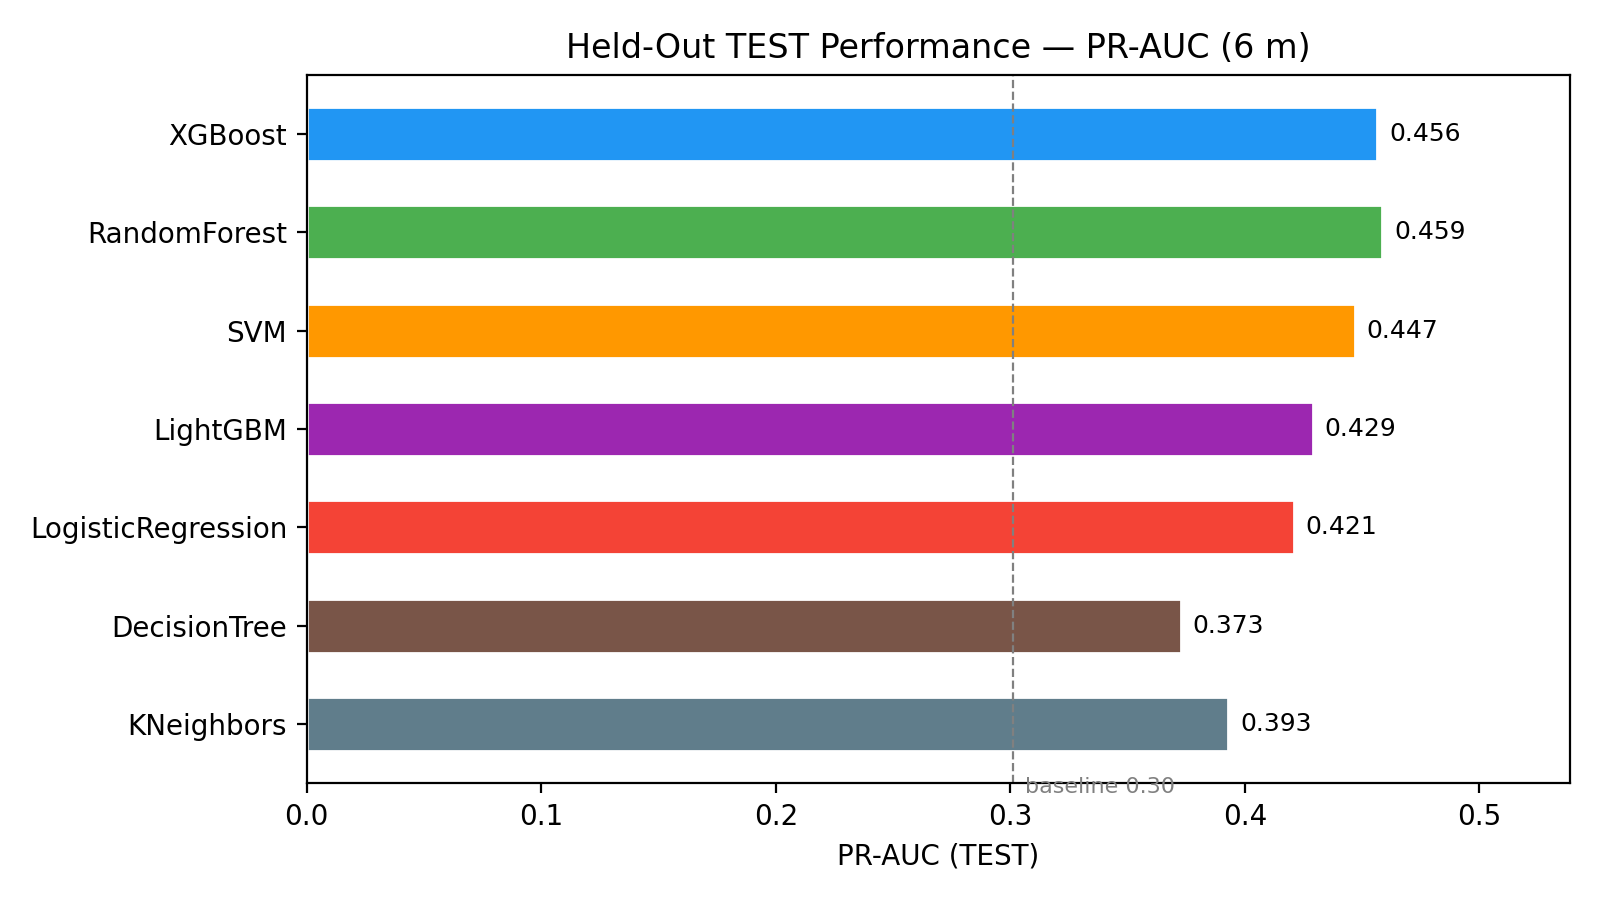
\includegraphics[width=0.82\linewidth]{images/figures/step6_test_prauc_bar.png}
  \caption[TEST set PR-AUC by model]{PR-AUC on the held-out TEST set (6\,m) for the seven best-per-family models.
  The dashed line indicates the baseline prevalence (0.30).}
  \label{fig:step6_test_prauc_bar}
\end{figure} 

\subsection{PR and ROC Curves}

Figures~\ref{fig:step6_pr_curves} and~\ref{fig:step6_roc_curves} present the precision--recall and ROC curves for all models on the TEST set.

\begin{figure}[ht!]
  \centering
  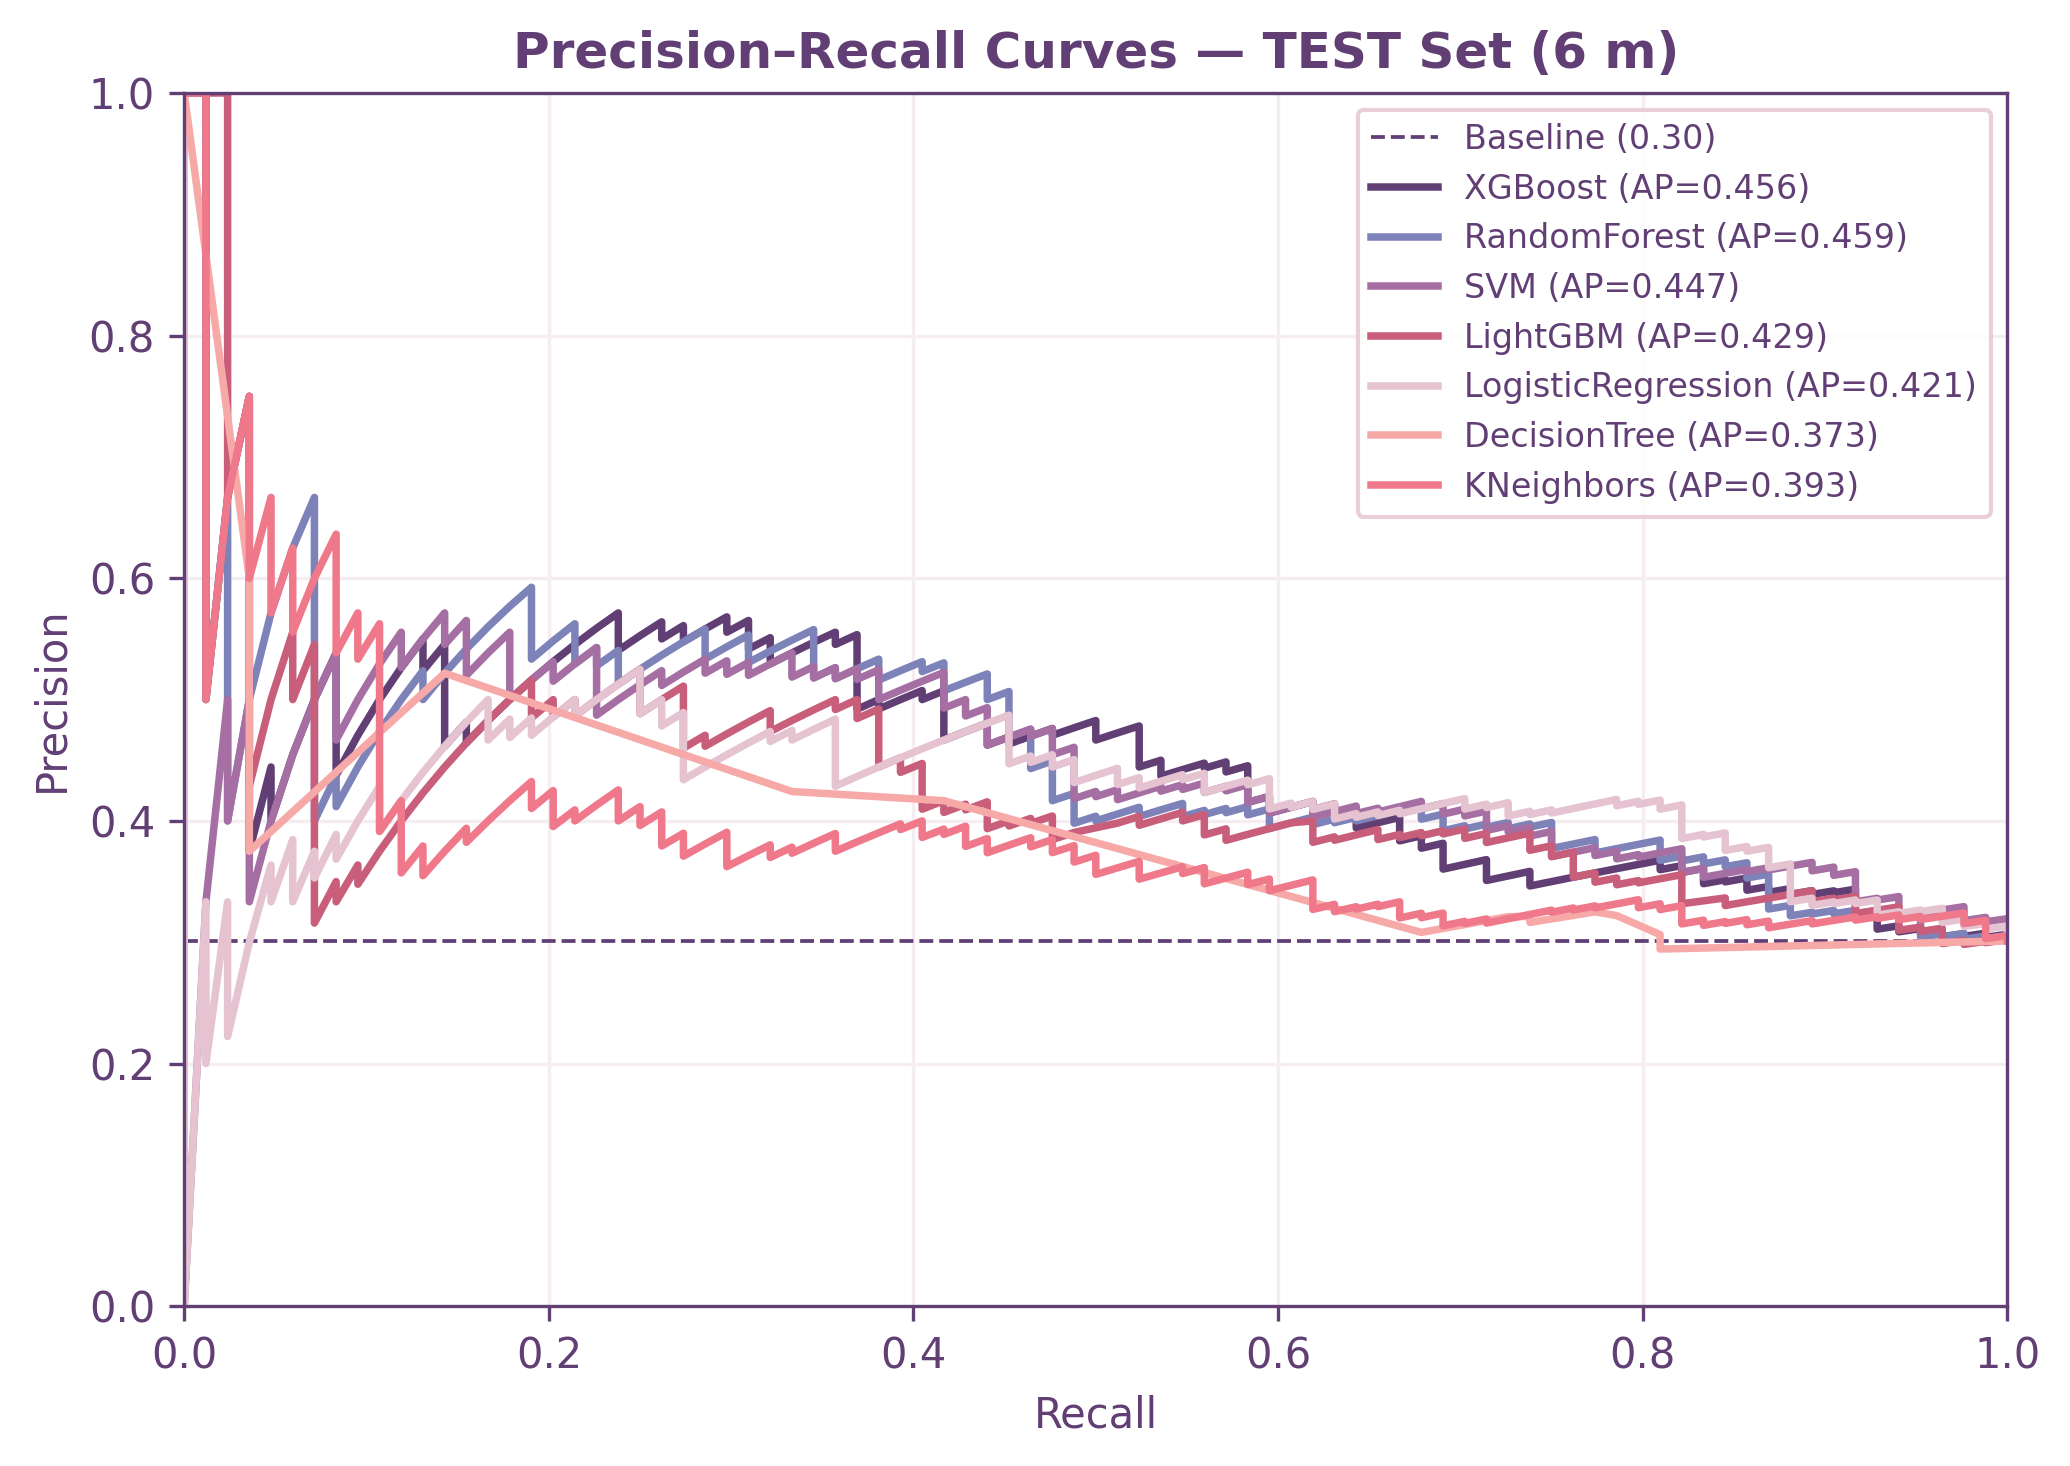
\includegraphics[width=0.82\linewidth]{images/figures/step6_pr_curves.png}
  \caption[Precision--Recall curves on TEST set]{Precision--Recall curves on the held-out TEST set (6\,m). The dashed line indicates the baseline prevalence ($0.30$).}
  \label{fig:step6_pr_curves}
\end{figure}

\begin{figure}[ht!]
  \centering
  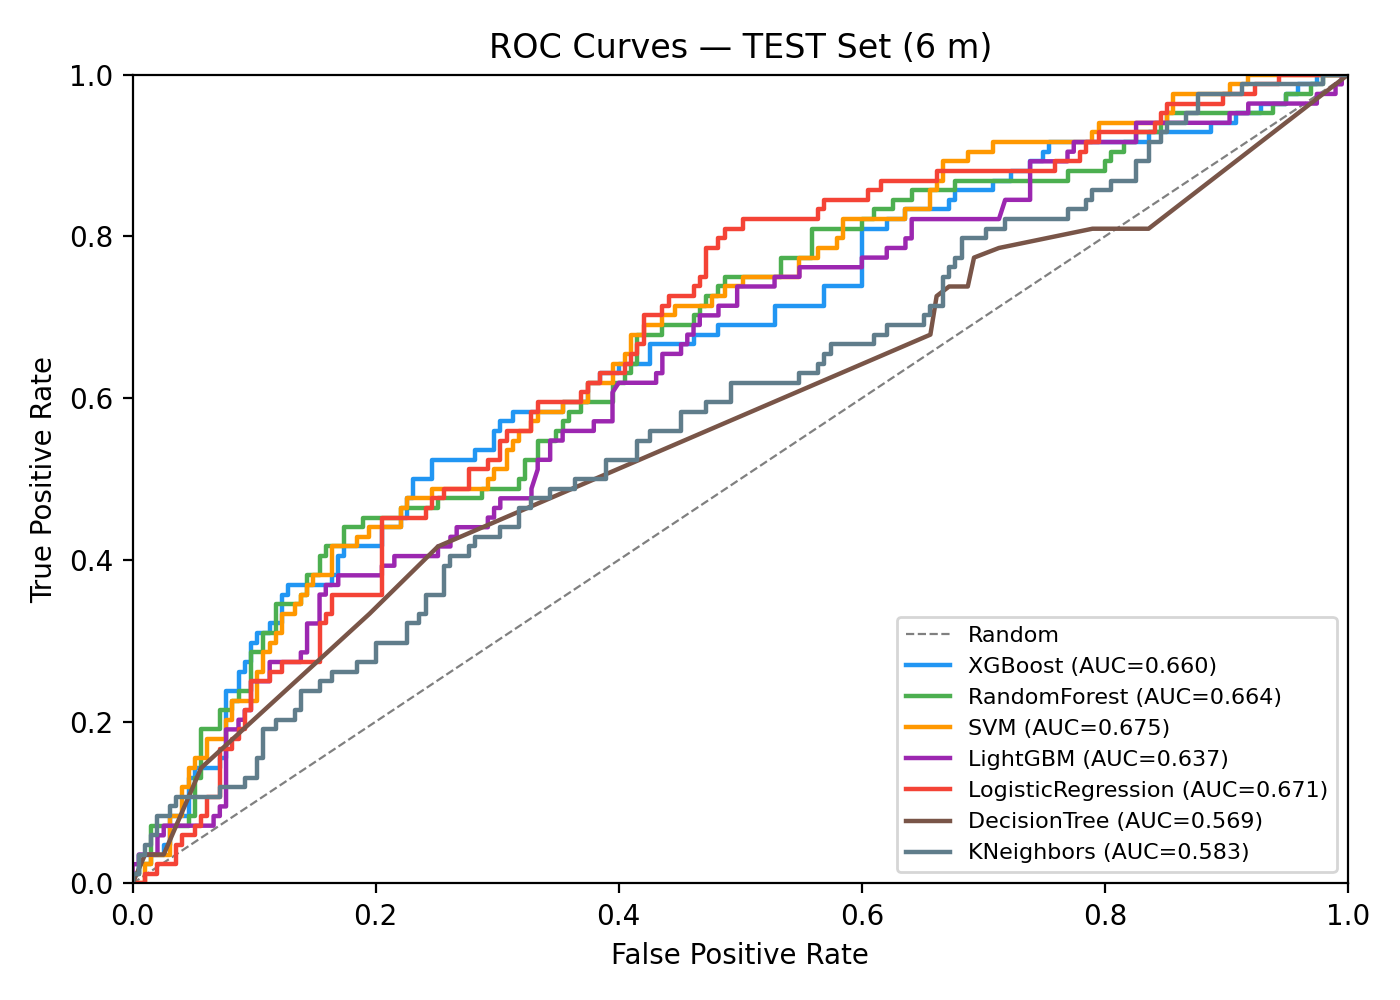
\includegraphics[width=0.82\linewidth]{images/figures/step6_roc_curves.png}
  \caption[ROC curves on TEST set]{ROC curves on the held-out TEST set (6\,m). The dashed line indicates the random classifier.}
  \label{fig:step6_roc_curves}
\end{figure}

\clearpage
\subsection{Threshold Evaluation on TEST}

$t=0.21$, selected from DEV OOF predictions (Section~\ref{sec:results_threshold_xgb}), is applied unchanged to the TEST set.
Table~\ref{tab:step6_threshold_test} compares XGBoost performance at multiple thresholds.

\begin{table}[ht!]
\centering
\caption[XGBoost performance at different thresholds]{DEV-fitted XGBoost (unbalanced, 6\,m) performance on TEST at different decision thresholds.}
\label{tab:step6_threshold_test}
\small
\begin{tabular}{c c c c c c c c c}
\toprule
$t$ & Precision & Recall & $F_1$ & $F_2$ & TP & FP & FN & TN \\
\midrule
0.21 & 0.351 & 0.857 & 0.498 & 0.665 & 72 & 133 & 12 & 62 \\
0.30 & 0.458 & 0.524 & 0.489 & 0.509 & 44 & 52  & 40 & 143 \\
0.35 & 0.500 & 0.405 & 0.447 & 0.421 & 34 & 34  & 50 & 161 \\
0.50 & 0.400 & 0.048 & 0.085 & 0.058 & 4  & 6   & 80 & 189 \\
\bottomrule
\end{tabular}
\end{table}

\noindent At the chosen threshold $t\!=\!0.21$:
\begin{itemize}
  \item The model identifies 72 of 84 rapid progressors (\textbf{recall\,$=\!85.7$\%}), missing only 12.
  \item It classifies 205 of 279 participants (73.5\%) as rapid. Of these, 133 are false positives, giving precision of 35.1\%.
  \item $F_1\!=\!0.498$ and $F_2\!=\!0.665$. Recall and precision are close to the corresponding DEV values, although this is a single held-out evaluation.
\end{itemize}

\noindent At the DEV-derived Youden threshold ($t\!=\!0.35$), TEST precision rises to 50.0\%, but recall falls to 40.5\%. The comparison illustrates the consequence of the selected operating point: $t=0.21$ retains substantially more rapid progressors at the cost of many additional false positives. Whether this trade-off is acceptable would require an externally defined clinical use case and prospective assessment; those conditions are not established in the present retrospective study.


\subsection{Calibration Analysis}

The probabilistic predictions of the DEV-fitted XGBoost model are examined using a reliability diagram and the Brier score (Figure~\ref{fig:step6_calibration}). Its Brier score is \textbf{0.197}, compared with approximately 0.210 for a constant prediction equal to the TEST prevalence. The reliability curve is close to the diagonal in the lower populated bins but departs from it at higher predicted probabilities, where fewer observations are available. The result indicates a modest reduction in mean squared probabilistic error relative to the constant reference, but does not demonstrate full calibration.

\begin{figure}[ht!]
  \centering
  
\includegraphics[width=0.55\linewidth]{images/figures/step6_calibration.png}
  \caption[XGBoost calibration on TEST set]{Reliability diagram for the DEV-fitted XGBoost model on TEST. The dashed line indicates perfect calibration; only probability bins containing observations are shown.}
  \label{fig:step6_calibration}
\end{figure}
\newpage
\subsection{Confusion Matrix}

Figure~\ref{fig:step6_cm} presents the confusion matrix at the $F_1$-optimal threshold ($t\!=\!0.21$).

\begin{figure}[H]
  \centering
  
\includegraphics[width=0.50\linewidth]{images/figures/step6_confusion_matrix.png}
  \caption[XGBoost confusion matrix at $t{=}0.21$]{Confusion matrix for the DEV-fitted XGBoost model on TEST at the DEV-derived threshold $t\!=\!0.21$.}
  \label{fig:step6_cm}
\end{figure}

\subsection{Post-Evaluation Refit}

After completion of the held-out evaluation and the TEST-based analyses reported in this chapter, the selected XGBoost pipeline is refitted on all 1,392 six-month participants for use by the prototype reporting workflow. This artefact uses the full-cohort slope cutoff ($-1.248$ points per 30 days) and retains the DEV-derived operating threshold $t=0.21$. A balanced Logistic Regression pipeline is refitted in parallel. No performance estimate is reported from these full-cohort fits, since they include the former TEST participants in training.

% ============================================================
\section{Explainability Analysis}
\label{sec:results_shap}
% ============================================================

This section examines the XGBoost model fitted on DEV using three complementary approaches: SHAP (global and local), LIME (local), and Logistic Regression coefficient analysis.
The XGBoost explanations are computed for the held-out TEST set ($N\!=\!279$), without refitting the model on those participants.

% ------------------------------------------------------------
\subsection{SHAP --- Global Explanations}
\label{subsec:results_shap_global}
% ------------------------------------------------------------

Figure~\ref{fig:shap_bar_global} ranks features by mean absolute SHAP value across all TEST-set subjects.
The baseline ALSFRS-R total score ranks first, with a mean $|\text{SHAP}|$ of \textbf{0.292}, more than twice that of FVC in litres (0.123).
Age (0.093), respiratory rate (0.086), pulse (0.073), ALT (0.061), and FVC as percentage of normal (0.054) follow.
The ranking indicates that functional and respiratory measurements carry most of the model's attribution magnitude, while variables from the other blocks make smaller contributions.

\begin{figure}[H]
  \centering
  
\includegraphics[width=0.85\linewidth]{images/figures/shap_bar_global.pdf}
  \caption[SHAP global feature importance, top 15]{Mean absolute SHAP values (top~15 features) for the DEV-fitted XGBoost model on the TEST set. Baseline ALSFRS-R total score ranks first, followed by FVC in litres and age.}
  \label{fig:shap_bar_global}
\end{figure}
\newpage
The beeswarm plot (Figure~\ref{fig:shap_beeswarm}) reveals the direction of these effects.
Lower ALSFRS-R scores generally shift predictions towards the rapid class, whereas higher scores tend to shift them towards the slow class.
Lower FVC values show a similar pattern.
The effects of age, respiratory rate, and the remaining variables are less uniform, which is compatible with non-linearities and interactions in the fitted model.

\begin{figure}[H]
  \centering
  
\includegraphics[width=0.85\linewidth]{images/figures/shap_beeswarm.pdf}
  \caption[SHAP beeswarm plot, XGBoost TEST set]{SHAP beeswarm plot for the DEV-fitted XGBoost model on TEST. Each dot represents one subject; colour indicates the observed feature value (red\,=\,high, blue\,=\,low). Positive SHAP values shift the prediction towards the rapid class.}
  \label{fig:shap_beeswarm}
\end{figure}

\clearpage
% ------------------------------------------------------------
\subsection{SHAP --- Local Explanations (Case Studies)}
\label{subsec:results_shap_local}
% ------------------------------------------------------------

One subject was selected from each confusion-matrix quadrant by choosing the case closest to the median predicted probability within that quadrant. This avoids selecting unusually confident predictions. The true positive and false negative are retained here to contrast a correctly detected rapid progressor with one missed at the same operating threshold. Profiles for all four subjects and the remaining local explanations are reported in Appendix~\ref{app:local_explanations}.

\noindent\textbf{True Positive (Subject~672752).}
Figure~\ref{fig:shap_wf_tp} shows the SHAP waterfall for this correctly identified rapid progressor.
The high ALSFRS-R score (43) shifts the prediction towards the slow class.
This is offset by respiratory rate, the imputed FVC value, temperature, and several smaller contributions, leaving the predicted probability above the operating threshold.

\begin{figure}[H]
  \centering
  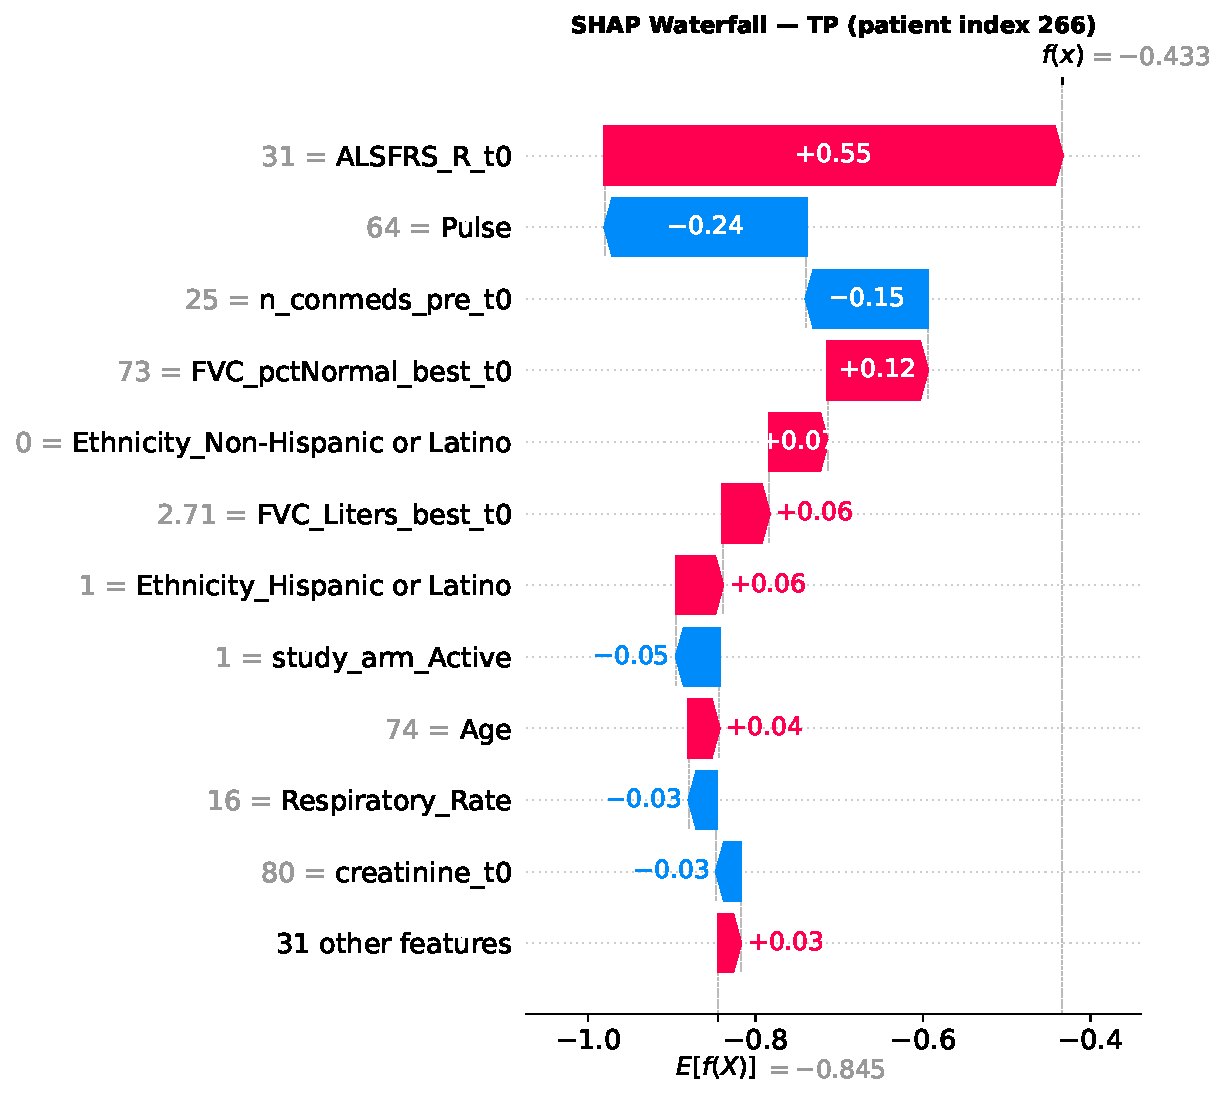
\includegraphics[width=0.63\linewidth]{images/figures/shap_waterfall_TP.pdf}
  \caption[SHAP waterfall: true positive case (Subject 672752)]{SHAP waterfall plot for the TP case study (Subject~672752). Respiratory rate and several smaller contributions offset the effect of a high baseline ALSFRS-R score. The horizontal scale is the XGBoost raw margin (log-odds) for rapid progression; the corresponding probability is reported in Table~\ref{tab:case_study_profiles}.}
  \label{fig:shap_wf_tp}
\end{figure} \break

\noindent\textbf{False Negative (Subject~330379).}
This rapid progressor was missed by the model (Figure~\ref{fig:shap_wf_fn}).
Low ALT, an ALSFRS-R score of 39, temperature, and several smaller effects shift the prediction towards the slow class, resulting in a probability of 0.169.
The case illustrates that the baseline profile can appear insufficiently suggestive of the decline observed during follow-up.

\begin{figure}[H]
  \centering
  
\includegraphics[width=0.62\linewidth]{images/figures/shap_waterfall_FN.pdf}
  \caption[SHAP waterfall: false negative case (Subject 330379)]{SHAP waterfall plot for the FN case study (Subject~330379). The combined baseline contributions shift the prediction below the selected threshold. The horizontal scale is the XGBoost raw margin (log-odds) for rapid progression; the corresponding probability is reported in Table~\ref{tab:case_study_profiles}.}
  \label{fig:shap_wf_fn}
\end{figure}

\clearpage
% ------------------------------------------------------------
\subsection{LIME --- Local Explanations}
\label{subsec:results_lime}
% ------------------------------------------------------------

LIME was applied to the same four subjects, using 2{,}000 perturbations per case to fit a sparse local surrogate. The resulting explanations provide a methodologically different view of the same predictions; the four plots are presented in Appendix~\ref{app:local_lime}.
% ------------------------------------------------------------
\subsection{SHAP--LIME Concordance}
\label{subsec:results_concordance}
% ------------------------------------------------------------

The top-ten SHAP and LIME rankings share five to seven features across the four cases, corresponding to an overlap of 50--70\%. ALSFRS-R appears in every shared set, while age, FVC, respiratory rate, pulse, BMI, and temperature recur in individual cases. The remaining differences reflect what each method measures: TreeSHAP attributes the fitted tree model's output, whereas LIME approximates its decision surface around perturbed observations. The comparison is therefore descriptive agreement, not validation of either explanation. Appendix~\ref{app:local_concordance} reports the shared features for each case.

% ------------------------------------------------------------
\subsection{Logistic Regression Coefficients}
\label{subsec:results_lr_coefs}
% ------------------------------------------------------------

As a complementary, model-intrinsic explanation, we analyse the coefficients of the balanced Logistic Regression model (Figure~\ref{fig:lr_coefs}).
Numeric features are standardised prior to fitting, whereas one-hot encoded indicators remain binary; coefficient magnitudes are therefore most directly comparable within the same feature type.

\begin{figure}[ht!]
  \centering
  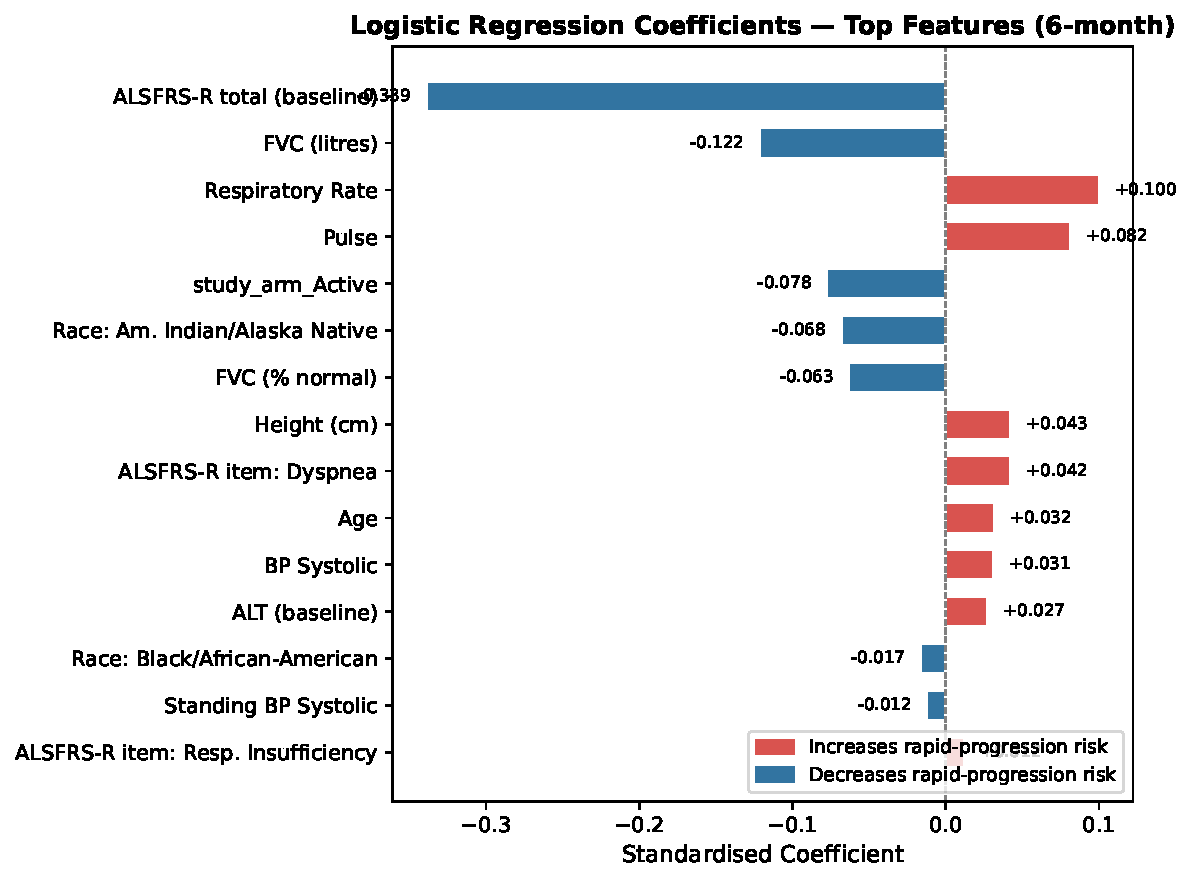
\includegraphics[width=0.85\linewidth]{images/figures/lr_coefficients.pdf}
  \caption[Logistic regression coefficients]{Coefficients of the balanced Logistic Regression model (top~15 by absolute value). Numeric features are standardised before fitting, while one-hot encoded indicators remain binary. Negative coefficients (blue) reduce the predicted log-odds of rapid progression; positive coefficients (red) increase them.}
  \label{fig:lr_coefs}
\end{figure}
\newpage
\noindent The top three LR coefficients by absolute value are:
\begin{enumerate}
  \item \textbf{ALSFRS-R\_t0} ($\beta = -0.283$): higher baseline function is associated with lower predicted log-odds of rapid progression.
  \item \textbf{Respiratory\_Rate} ($\beta = +0.115$): higher respiratory rate is associated with higher predicted log-odds.
  \item \textbf{FVC\_Litres} ($\beta = -0.088$): higher forced vital capacity is associated with lower predicted log-odds.
\end{enumerate}

\noindent Functional status and respiratory measurements therefore recur in both the linear and non-linear models, although their exact ranking differs.
Age ($\beta = +0.076$), study-arm assignment ($\beta = -0.062$), FVC percentage of normal ($\beta = -0.052$), temperature ($\beta = -0.050$), and pulse ($\beta = +0.045$) also appear among the larger Logistic Regression coefficients.

\subsection{Summary of Explainability Findings}
\label{subsec:results_xai_summary}

Baseline ALSFRS-R carries the largest global SHAP importance and the largest absolute Logistic Regression coefficient. FVC and respiratory rate also recur in both models and in several local explanations, while age, pulse, and temperature provide smaller predictive signals. The agreement across model families is strongest for baseline function and respiratory status rather than for every individual feature.

The local cases show why this agreement does not make each prediction reliable. For the selected false negative, several baseline measurements push the probability below the threshold even though the participant later meets the rapid-progression definition. SHAP and LIME share 50--70\% of their ten highest-ranked features across the four cases, but their differences remain relevant because the methods explain the prediction in different ways.


% ============================================================
\section{Supplementary Analyses}
\label{sec:results_supplementary}
% ============================================================

This section presents six supplementary analyses of the DEV-fitted XGBoost model: error profiling, subgroup performance, decision curve analysis, learning curves, bootstrap confidence intervals, and partial dependence plots.
All analyses use the held-out TEST set ($N\!=\!279$) at the $F_1$-optimal threshold $t\!=\!0.21$.

% ------------------------------------------------------------
\subsection{Error Profiling}
\label{subsec:results_error_profile}
% ------------------------------------------------------------

At $t=0.21$, the model misses 12 of 84 rapid progressors and produces 133 false positives. Seven false negatives have a baseline \gls{ALSFRS-R} score of at least 40, including five in the mildest group ($>42$), while six occur among participants aged 49 years or younger. False-negative proportions are similar for female and male participants (4.7\% and 4.0\%), and the incomplete \gls{FVC} data do not support a clear respiratory pattern. The concentration of missed cases among participants with relatively preserved baseline function motivates the subgroup analysis that follows. Appendix~\ref{app:error_profiles} contains the four stratified error profiles and their detailed interpretation.

% ------------------------------------------------------------
\subsection{Subgroup Performance}
\label{subsec:results_subgroup}
% ------------------------------------------------------------

Baseline functional status shows the clearest subgroup variation. Recall falls from 97.2\% among participants with \gls{ALSFRS-R} $\leq35$ to 54.5\% in the $>42$ group; these estimates are based on 36 and 11 rapid progressors, respectively. The youngest age group also has lower recall than the overall \gls{TEST} value (72.7\% versus 85.7\%). Female and male participants have similar point estimates for PR-AUC (0.450 and 0.473) and recall (84.4\% and 86.5\%), although no formal equivalence or fairness test was performed.

PR-AUC varies across the \gls{FVC} strata, but the lower-FVC groups also contain a higher proportion of rapid progressors. The metric differences therefore cannot be separated from subgroup prevalence in this analysis. Appendix~\ref{app:subgroup_performance} reports all strata, including participants with missing age or FVC, together with the complete table and figures.

% ------------------------------------------------------------
\subsection{Decision Curve Analysis}
\label{subsec:results_dca}
% ------------------------------------------------------------

The model has higher estimated net benefit than both reference strategies across the main continuous interval $t\in[0.18,\,0.47]$. At the selected operating point ($t=0.21$), net benefit is 0.131, compared with 0.115 for treat all and 0 for treat none. The difference from treat all corresponds to approximately 1.6 additional net true-positive decisions per 100 participants under the threshold-implied weighting of false positives. This is evidence of potential decision value within the evaluated sample, not established clinical utility: no intervention has been specified, the analysis lacks uncertainty intervals, and external validation has not been performed. Appendix~\ref{app:dca} presents the full curve and isolated threshold results.

% ------------------------------------------------------------
\subsection{Learning Curves}
\label{subsec:results_learning_curves}
% ------------------------------------------------------------

Mean PR-AUC increases from 0.424 with 20\% of \gls{DEV} ($n=222$) to 0.446 with 90\% ($n=1{,}001$), while the standard deviation across repeated subsets decreases from 0.029 to 0.011. The model fitted once on all 1{,}113 development participants reaches 0.456. Since adjacent error bars generally overlap and the mean curve is not monotonic, the analysis indicates modest gains and greater stability with more training data but does not locate a clear performance plateau. The deterministic full-data point is not directly comparable with the repeated-subset variation, nor can this experiment predict the benefit of a larger independent cohort. Appendix~\ref{app:learning_curve} presents the complete curve.

% ------------------------------------------------------------
\subsection{Bootstrap Confidence Intervals}
\label{subsec:results_bootstrap}
% ------------------------------------------------------------

Table~\ref{tab:bootstrap_ci} and Figure~\ref{fig:bootstrap_ci} present 95\% bootstrap confidence intervals ($B\!=\!2{,}000$) for the key TEST-set metrics.

\begin{table}[ht!]
\centering
\caption[Bootstrap 95\% confidence intervals, TEST set]{Bootstrap 95\% confidence intervals for TEST-set metrics ($B\!=\!2{,}000$, $t\!=\!0.21$).}
\label{tab:bootstrap_ci}
\small
\begin{tabular}{l c c c}
\toprule
\textbf{Metric} & \textbf{Point estimate} & \textbf{95\% CI} & \textbf{CI width} \\
\midrule
PR-AUC    & 0.456 & [0.364,~0.568] & 0.204 \\
ROC-AUC   & 0.660 & [0.586,~0.730] & 0.144 \\
Recall    & 0.857 & [0.781,~0.929] & 0.148 \\
Precision & 0.351 & [0.283,~0.419] & 0.136 \\
$F_1$     & 0.498 & [0.423,~0.568] & 0.145 \\
$F_2$     & 0.665 & [0.593,~0.729] & 0.136 \\
Brier     & 0.197 & [0.174,~0.221] & 0.047 \\
\bottomrule
\end{tabular}
\end{table}

\begin{figure}[ht!]
  \centering
  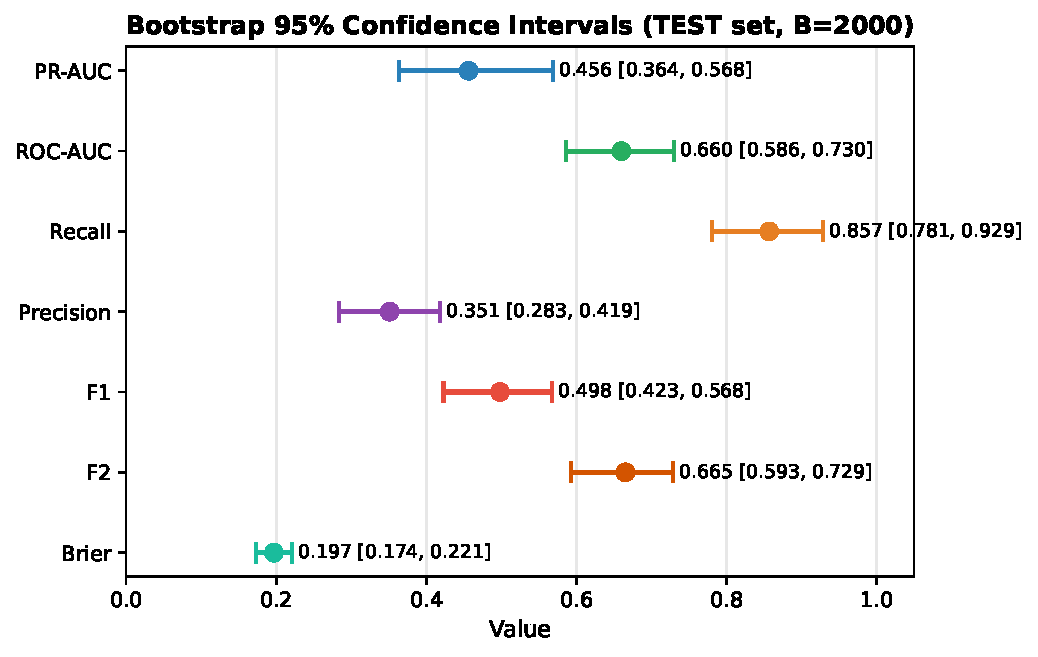
\includegraphics[width=0.78\linewidth]{images/figures/bootstrap_ci.pdf}
  \caption[Forest plot of bootstrap confidence intervals]{Forest plot of percentile-bootstrap 95\% confidence intervals for TEST-set metrics ($B\!=\!2{,}000$). The intervals describe TEST-sample uncertainty conditional on the fitted model and fixed threshold.}
  \label{fig:bootstrap_ci}
\end{figure}
\newpage
\noindent\textbf{Key observations:}
\begin{itemize}
  \item PR-AUC has the widest interval, $[0.364,\,0.568]$, showing appreciable uncertainty around the point estimate of 0.456.
  \item Recall is estimated at 0.857 with a 95\% interval of $[0.781,\,0.929]$. The corresponding $F_2$ interval is $[0.593,\,0.729]$, reflecting uncertainty in screening-oriented threshold performance.
  \item Precision remains comparatively low across the bootstrap distribution, with an interval of $[0.283,\,0.419]$, consistent with the large number of false positives at $t=0.21$.
  \item The Brier interval is $[0.174,\,0.221]$. Its smaller numerical width is not directly comparable with those of discrimination or classification metrics because the measures have different sampling distributions and interpretations.
  \item These intervals quantify variation from resampling TEST participants only. They should not be read as covering the additional uncertainty introduced by model development and threshold selection.
\end{itemize}

% ------------------------------------------------------------
\subsection{Partial Dependence Plots}
\label{subsec:results_pdp}
% ------------------------------------------------------------

The marginal prediction decreases across the observed baseline \gls{ALSFRS-R} range of 29--46, with step changes characteristic of a tree ensemble. For \gls{FVC}, the curve is relatively flat below approximately 3.7 litres, falls around 3.8--4.0 litres, and then stabilises. The age curve rises around the low 40s before remaining broadly stable across most higher values. These patterns complement the global \gls{SHAP} ranking by describing the model's average response shape.

The curves remain descriptive. FVC in litres is observed for only 162 of 279 \gls{TEST} participants, and age for 246; correlations between baseline function, respiratory measurements, age, and other covariates also mean that some combinations evaluated by the PDP may be uncommon in the cohort. Appendix~\ref{app:pdp} presents the full figure, observed-value density, and PDP ranges.

% ============================================================
\section{Patient Risk Report}
\label{sec:results_patient_report}
% ============================================================

The generator described in Section~\ref{sec:methods_patient_report} produced complete reports for 12 cohort records and ten fictitious profiles. Baseline \gls{ALSFRS-R} was the largest absolute \gls{SHAP} contributor in nine of the 12 cohort examples, whereas the fictitious inputs produced a wider mix of leading features. These runs verified the path from input data to prediction, local explanation, and formatted output. They do not provide an additional performance estimate: the cohort records were seen during the final full-cohort refit, and the fictitious profiles do not preserve the clinical data's joint distribution. Appendix~\ref{app:patient_report} describes the demonstrator and reports the example outputs in full.

% ============================================================
\section{Summary of Key Findings}
\label{sec:results_summary}
% ============================================================

Study~I examined whether rapid six-month functional progression could be predicted from baseline \gls{PRO-ACT} data under a leakage-free evaluation protocol.
Its main findings can be summarised as follows:

\begin{enumerate}
  \item \textbf{The cohort supported the intended analysis, but data quality required active review.}
    The six-month cohort included 1,392 participants, and 99.8\% of the slopes were estimated from at least three \gls{ALSFRS-R} measurements.
    The preprocessing audit identified a systematic height-unit error affecting 147 raw records, 132 of which reached the selected feature set, and showed that \gls{FVC} availability varied across trials.
    The source of the missingness could not be established from the available data.

  \item \textbf{No single classifier was clearly superior.}
    Among 13 tuned configurations, unbalanced XGBoost ranked first on development \gls{PR-AUC} ($0.434 \pm 0.049$), narrowly ahead of unbalanced Random Forest ($0.431 \pm 0.042$) and balanced \gls{SVM} ($0.425 \pm 0.049$).
    The fold-level distributions overlapped, and the Friedman test did not reject equal model ranks ($p=0.053$).
    XGBoost was therefore selected by the prespecified ranking rule, not because statistical superiority had been demonstrated.

  \item \textbf{Baseline functional status contained most of the predictive signal.}
    The core feature block retained most of the cross-validated performance, while adding \gls{FVC} gave the clearest incremental gain for Random Forest and XGBoost.
    Vital signs, treatment variables, and laboratory measurements had smaller and less consistent effects.
    Repeating the analysis at three months produced a similar range of \gls{PR-AUC} values, although the model ordering changed slightly; six months remained the primary horizon because the slopes were supported by longer follow-up.

  \item \textbf{Held-out discrimination was moderate and uncertain.}
    The selected XGBoost model achieved a TEST \gls{PR-AUC} of 0.456, compared with a rapid-progression prevalence of 0.301.
    Random Forest was almost identical at 0.459, but the held-out partition was not used to reopen model selection.
    The bootstrap 95\% interval for XGBoost \gls{PR-AUC} was wide ($[0.364,\,0.568]$), and the Brier score of 0.197 indicated modest probabilistic accuracy rather than full calibration.

  \item \textbf{The operating threshold determined the practical behaviour of the model.}
    At the development-derived threshold of $t=0.21$, XGBoost detected 72 of 84 rapid progressors on TEST (recall 85.7\%) but classified 205 of 279 participants as rapid.
    Precision was 35.1\%, with 133 false positives, showing that the gain in sensitivity came at a substantial cost in specificity.
    The threshold is consequently an experimental, sensitivity-oriented operating point rather than a clinically established cutoff.

  \item \textbf{The explanations were coherent at population level but less uniform for individual records.}
    Baseline \gls{ALSFRS-R} had the largest global SHAP contribution, followed by \gls{FVC}, age, and respiratory rate; Logistic Regression gave a compatible overall ranking.
    Local SHAP and \gls{LIME} shared 50--70\% of their top-ten features across the four case studies, which supports partial agreement but not interchangeability.
    Error profiling exposed a threshold-specific limitation: recall fell to 54.5\% in the mildest baseline \gls{ALSFRS-R} subgroup ($>42$), where five of the 12 false negatives occurred.

  \item \textbf{The supplementary analyses support further investigation, not clinical use.}
    Decision Curve Analysis estimated positive net benefit relative to both reference strategies across the main interval $t\in[0.18,\,0.47]$, while the learning curves did not show a clear performance plateau.
    Partial dependence patterns and the patient-level report provide additional views of model behaviour, but neither establishes causal effects, external validity, or readiness for individual clinical decisions.
\end{enumerate}

\bigskip
\noindent
Study~I therefore provides a reproducible framework for short-term functional progression prediction rather than a model ready for deployment.
Its main contribution lies in the complete evaluation protocol: temporally valid target construction, subject-wise validation, metric-led model selection, development-only threshold choice, held-out testing, and post-hoc explanation.
The distinction between ranking performance and threshold-dependent behaviour becomes particularly important in Study~II, where the class imbalance is more severe and the target changes from functional decline to survival.
That study is described in Chapter~\ref{ch:study2_methods}.
